%====================================================
%	CHAPTER 4 - Control
%====================================================
\chapter{Controller Development}
\label{ch:control}
%====================================================
\section{Stability}
\label{sec:control.stability}
%====================================================
Before embarking on control plant derivations, it is worth outlining definitions of what the control objectives are. The research question is posed as dynamic set-point tracking, the system's control loop then aims to \emph{stabilize} the dynamics described previously in Sec:\ref{sec:dynamics.model} whilst tracking particular trajectories for attitude and position, or tracking a state set-point $\mathbf{x}_d=[\vec{\mathcal{E}}_d~Q_d]^T$. 
\par
Each control block within the loop is expanded upon subsequently in Sec:\ref{sec:control.loop} but first; stability in the context of trajectory tracking must be defined. Stability definitions for a generealized plant trajectory are not uncommon in the context of energy equation control proofs (see Sec:\ref{sec:control.lyapunov}) and are discussed in most control texts. Only stability definitions pertinent to Lyapunov's stability theorem are briefly presented here; the following is adapted from \cite{bojelayupanov,lyapunovstabilitytheorem}. In general for some autonomous trajectory $\vec{\mathbf{x}}(t)$, an equilibrium point $\vec{\mathbf{x}}(t_0)$ is said to be stable (\textbf{S}) if and only if (\emph{iff}) the following is true:
\begin{subequations}\label{eq:basic-stability}
\begin{equation}
\forall\varepsilon>0,~\exists~\delta_0(t_0,\varepsilon):~\norm{\vec{\mathbf{x}}(t_0)}<\delta_0(t_0,\varepsilon)
\end{equation}
\vspace{-20pt}
\begin{equation}
\Rightarrow\norm{\vec{\mathbf{x}}(t)}<\varepsilon,~~\forall t\geq t_0
\end{equation}
\end{subequations}
The implication of which is that if, for some initial condition $\vec{\mathbf{x}}(t_0)$ whose magnitude is bound by the manifold $\delta_0(t_0,\varepsilon)$, the entire subsequent trajectory of $\vec{\mathbf{x}}(t)$ is bound from above by some other manifold $\varepsilon$. Such a trajectory is illustrated for a two dimensional case in Fig:\ref{fig:basic-stability}.
\begin{figure}[hbtp]
\vspace{-6pt}
\centering
\begin{subfigure}{0.49\textwidth}
\centering
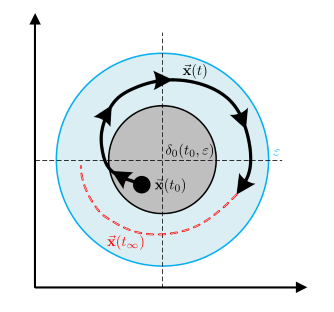
\includegraphics[width=\textwidth]{figs/basic-stability}
\vspace{-14pt}
\caption{Basic stability}
\label{fig:basic-stability}
\end{subfigure}
\begin{subfigure}{0.49\textwidth}
\centering
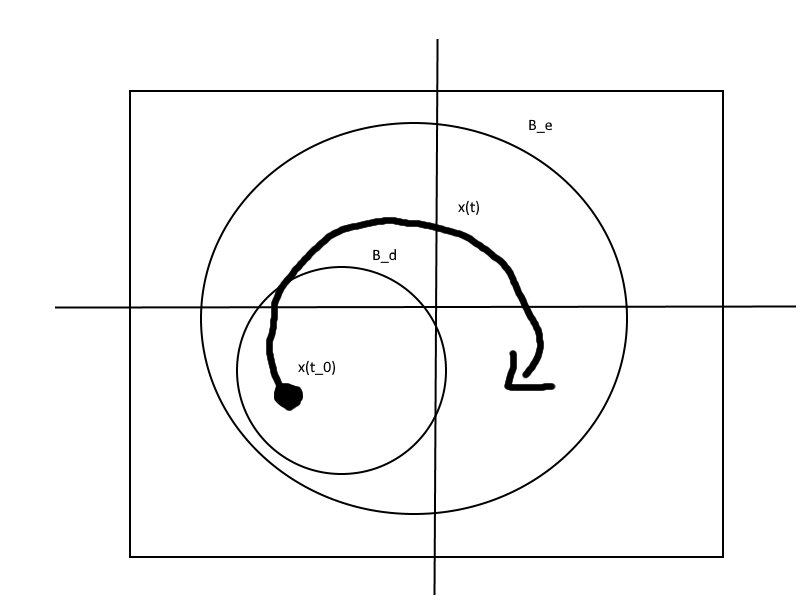
\includegraphics[width=\textwidth]{figs/uniform-stability}
\vspace{-14pt}
\caption{Uniform stability}
\label{fig:uniform-stability}
\end{subfigure}
\vspace{-4pt}
\caption{Trajectory illustrations for $\mathbf{S}$ and $\mathbf{US}$}
\vspace{-6pt}
\end{figure}
\par
An equilibrium point is further said to be uniformly stable (\textbf{US}) \emph{iff} for the time line $t\in[t_0,\infty)$ the following, an extension of basic stability, holds true:
\begin{subequations}\label{eq:uniform-stability}
\begin{equation}
\forall\varepsilon>0,~\exists~\delta_0(\varepsilon)>0:~\norm{\vec{\mathbf{x}}(t_1)}<\delta_0(\varepsilon),~~t_1>t_0
\end{equation}
\vspace{-14pt}
\begin{equation}
\Rightarrow\norm{\vec{\mathbf{x}}(t)}<\varepsilon,~~\forall
t\geq t_1
\end{equation}
\end{subequations}
\textbf{US} similarly bounds a trajectory from above by a manifold $\varepsilon$ if such a trajectory originates from within $\delta_0(\varepsilon)$. The difference is that the principle trajectory region $\delta_0(\varepsilon)$ is independent of $t_0$ in the case of \textbf{US}. The two surfaces can effectively be regarded as non-concentric; a $\mathbf{US}$ trajectory is illustrated in Fig:\ref{fig:uniform-stability}. 
\par
%============================================================
Uniform stability is a subset of general stability, $\mathbf{US}\subset\mathbf{S}$, however the converse is not true. Furthermore \textbf{US} is a stronger assertion of stability. Extending stability definitions to include settling; an equilibrium point is said to be asymptotically stable (\textbf{AS}) \emph{iff} conditions for \textbf{S} are met (Eq:\ref{eq:basic-stability}) and that the following holds true:
\begin{subequations}
\begin{equation}
\exists~\delta_1(t_0,\varepsilon) >0:~\norm{\vec{\mathbf{x}}(t_0)}<\delta_1(t_0,\varepsilon)
\end{equation}
\vspace{-12pt}
\begin{equation}
\Rightarrow \lim_{t\rightarrow\infty}\norm{\vec{\mathbf{x}}(t)}\rightarrow 0
\end{equation}
\end{subequations}
This implies that for trajectories originating from some finer region $\delta_1(t_0,\varepsilon)$, typically a subset of $\delta(t_0,\varepsilon)$, the trajectory tends to and \emph{asymptotically} settles at the origin. This means that in the case of \textbf{AS} the origin is both \underline{stable} and \underline{attractive} (shown in Fig:\ref{fig:asymptotic-stability}). Asymptotic stability is typically the first requirement for controllers, being a stronger stability than both \textbf{US} and \textbf{S}\ldots
\begin{figure}[hbtp]
\centering
\begin{subfigure}{0.49\textwidth}
\centering
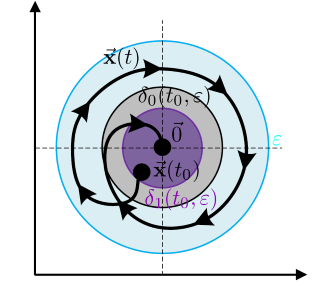
\includegraphics[width=\textwidth]{figs/asymptotic-stability}
\vspace{-8pt}
\caption{Asymptotic stability}
\label{fig:asymptotic-stability}
\end{subfigure}
\begin{subfigure}{0.49\textwidth}
\centering
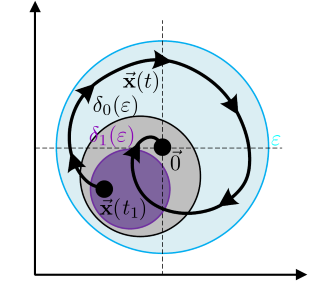
\includegraphics[width=\textwidth]{figs/uniform-asymptotic-stability}
\vspace{-8pt}
\caption{Uniform asymptotic stability}
\label{fig:uniform-asymptotic-stability}
\end{subfigure}
\vspace{-4pt}
\caption{Trajectory illustrations for $\mathbf{AS}$ and $\mathbf{UAS}$}
\vspace{-14pt}
\end{figure}
\par
Uniform asymptotic stability (\textbf{UAS}), an extension of uniform stability, occurs when the asymptotically stable bound region $\delta_1(\epsilon)$ is independent of the principle starting $t_0$. An equilibrium point is \textbf{UAS} \emph{iff} conditions for \textbf{S} are met and that:
\begin{subequations}
\begin{equation}
\exists~\delta_1(\varepsilon)>0:~\norm{\vec{\mathbf{x}}(t_1)}<\delta_1(\varepsilon),~~t_1\geq t_0
\end{equation} 
\vspace{-12pt}
\begin{equation}
\Rightarrow \lim_{t\rightarrow\infty}\norm{\vec{\mathbf{x}}(t)}\rightarrow 0
\end{equation}
\end{subequations}
A uniformly asymptotic equilibrium point implies stability from a non-concentric ball of attraction; settling to the origin (illustrated in Fig:\ref{fig:uniform-asymptotic-stability}).
\par
An equilibrium point is regarded as exponentially stable (\textbf{UES}) if conditions for \textbf{UAS} are met and that there exist $\exists~a,b,r$ that bound the settling of the trajectory such that:
\begin{equation}\label{eq:exponential-stability}
\norm{\vec{\mathbf{x}}(t,t_0,\vec{\mathbf{x}}_0)}\leq a\norm{\vec{\mathbf{x}}_0}e^{-bt},~~\forall\norm{\vec{\mathbf{x}}_0}\leq r
\end{equation}
The term $a\norm{\vec{\mathbf{x}}_0}e^{-bt}$ bounds the rate at which the trajectory settles to the origin, illustrated in Fig:\ref{fig:exponential-stability}. The initial point of the trajectory, $\vec{\mathbf{x}}_0$ is bound from above by some $r\triangleq \delta_1(\varepsilon)$. Uniform stability is implied with exponential stability\ldots
\begin{figure}[hbtp]
\centering
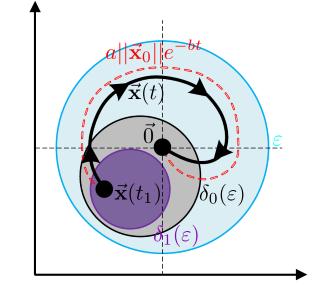
\includegraphics[width=0.5\textwidth]{figs/exponential-stability}
\vspace{-8pt}
\caption{Exponential stability, $\mathbf{UES}$}
\label{fig:exponential-stability}
\vspace{-14pt}
\end{figure}
\par
The above definitions of stability are only locally defined, and so the stabilities hold true only for local trajectories. Extending \textbf{UAS} to global uniform asymptotic stability (\textbf{GUAS}); the origin's equilibrium point is \textbf{GUAS} \emph{iff} conditions for \textbf{UAS} are first met, the origin is only the equilibrium point and the asymptotic approach can be extended such that:
\begin{subequations}
\begin{equation}
\exists~\delta_1(\varepsilon)>0:~\norm{\vec{\mathbf{x}}(t_1)}<\delta_1(\varepsilon),~~t_1\geq t_0
\end{equation}
\vspace{-16pt}
\begin{equation}
\Rightarrow \lim_{t\rightarrow\infty}\norm{\vec{\mathbf{x}}(t)},~~\forall \vec{\mathbf{x}}(t_0)
\end{equation}
\end{subequations}
Exponential stability can similarly be extended to the global case \emph{iff} \textbf{UES} conditions are first met. In the global case, the origin can be the only equilibrium point moreover conditions from Eq:\ref{eq:exponential-stability} are extended such that:
\begin{equation}\label{eq:global-exponential-stability}
\norm{\vec{\mathbf{x}}(t,t_0)}\leq a\norm{\vec{\mathbf{x}}_0}e^{-bt},~~\forall\norm{\vec{\mathbf{x}}_0}
\end{equation}
The conditions for the initial equilibrium point are dropped in Eq:\ref{eq:global-exponential-stability}; it follows that irrespective of the starting point for the trajectory, the system \underline{always} settles to the origin. \textbf{GUES} is the strongest sense of stability and further provides insight into the rate at which the trajectory stabilizes. The most effective control design outcome is a controller which applies globally uniform exponential stability to a plant.
%====================================================
\section{Control Loop}
\label{sec:control.loop}
%====================================================
The control problem for this dissertation is, as outlined in Ch:\ref{ch:intro}; to achieve dynamic (\emph{attitude and position}) set point tracking on a quadrotor by solving the problem of its inherent under-actuation through over-actuation. For the purposes of the subsequent controller development, the plant is described in the following typical non-linear state space form:
\begin{subequations}
\begin{equation}
\frac{d}{dt}{\vec{\mathbf{x}}}=f(\vec{\mathbf{x}},t)+g(\vec{\mathbf{x}},\vec{\nu},t)
\end{equation}
\vspace{-15pt}
\begin{equation}
\vec{y} = c(\vec{\mathbf{x}},t)+d(\vec{\mathbf{x}},\vec{\nu},t)
\end{equation}
\end{subequations}
Where the internal plant dynamics are governed by $f(\vec{\mathbf{x}},t)$ and the plant's input response by $g(\vec{\mathbf{x}},\vec{\nu},t)$, for a given control input $\vec{\nu}$. The latter could take the affine form; $g(\mathbf{x},t)\vec{\nu}$. Setpoint tracking aims for the output to track the plant's state; namely $\vec{y} = c(\vec{\mathbf{x}},t)=\vec{\mathbf{x}}$. As such, the control problem is to design a stabilizing control law for some error state $\mathbf{x}_e$:
%============================================================
% Up to here
%============================================================
\begin{equation}
\vec{\nu}_d=h(\mathbf{x}_e,t)
\end{equation}
Such that the control plant is globally asymptotically stable or that $\lim_{t\rightarrow\infty}\mathbf{x}_e=0$. It is possible to combine attitude and position states into a single common trajectory state such that:
\\
\vspace{-5pt}
\begin{equation}
\mathbf{x}=\begin{bmatrix}
\vec{\mathcal{E}}\\
Q_b
\end{bmatrix}
\end{equation}
The body's trajectory is then fully described by $\mathbf{x}(t)$. Separate control laws are developed for attitude and position tracking and hence those states aren't combined. However for the purposes of discussing the control plant, a single major loop is considered. The designed control input, $\vec{\nu}_d$, is then implemented by actuator suite $u\in\mathbb{U}$ through its effectiveness function:
\\
\vspace{-5pt}
\begin{equation}
\nu_c=B(\mathbf{x},u,t)
\end{equation}
The exact relationship of the virtual control input and commanded input, $\nu_c\rightarrow\nu_d$, is governed by the allocation algorithm. That allocation function, $B^\dagger$, can be \emph{roughly} referred to as the effectiveness inverse\footnote{Direct (\emph{pseudo}) inversion is the typical allocation scheme.}. The actuator positions are then solved for, avoiding saturation, subject to some constraint:
\begin{equation}
\underset{\in\mathbb{U}}{u}=B^{\dagger}(\mathbf{x},\nu_d,t)
\end{equation}
The control allocation requirements and schemes are expanded upon subsequently in Sec:\ref{sec:control.allocation}. Multiple attitude controllers are presented whose stability is proven with Lyapunov$^\dagger$ stability theorem. Each controller is compared in the context of an over actuated quadrotor plant. Similarly a series of proposed allocation schemes are evaluated too. Those comparisons, their details and how controller efficacy and stability are evaluated is all presented next in Chapter:\ref{ch:simulation}. 
\newpage
A generalized over-actuated control loop is split into a series of cascaded control blocks, each with an individual function, as illustrated in Fig:\ref{fig:control-loop}. From the error state of the generated trajectory, $\mathbf{x}_e$, the control law designs a virtual control input, $\vec{\nu}_d$, which is cast as the argument to the allocation block. From the allocation law, $B^{\dagger}(\mathbf{x},\vec{\nu}_d,t)$, physical actuator positions are obtained; $u\in\mathbb{U}$. Those actuator positions effect a virtual plant input, $\vec{\nu}_c=B(\mathbf{x},u,t)$, which is an input to the state function's dynamics, Eq:\ref{eq:quaternion-states}. Not shown, but implied in Fig:\ref{fig:control-loop}, is the state derivative feedback of $\dot{\mathbf{x}}$ to the plant transfer function. Finally the output tracking state is estimated with some filtration paradigm, $\hat{\mathbf{x}}=A(\mathbf{x},t)$, and fed back to the error state.
\begin{figure}[htbp]
\centering
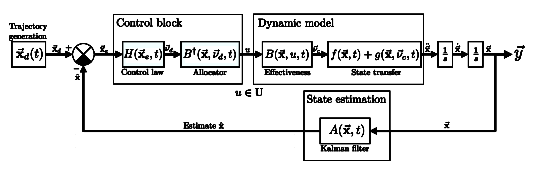
\includegraphics[width=0.95\textwidth]{figs/control-loop}
\caption{Generalized control loop with allocation}
\label{fig:control-loop}
\end{figure}
\vspace{-20pt}
%====================================================
\section{Control Plant Inputs}
\label{sec:control.inputs}
%====================================================
Thus far control plant inputs for the set of differential state equations, from Eq:\ref{eq:quaternion-states}, have mostly been described with net forces and torques; $\mu\vec{F}$ \& $\mu\vec{\tau}$. The relationship between each propeller's rotational speed \& servo positions and the its resultant output thrust direction is calculated as a quaternion transformation of produced lift force, as in Eq:\ref{eq:quaternion-inputs}.
\begin{subequations}\label{eq:control-input}
\begin{equation}
\mu\vec{F}(u)=\sum Q_{M_i}^*(\lambda_i,\alpha_i)\otimes T(\Omega_i)\otimes Q_{M_i}(\lambda_i,\alpha_i)~~~~\in\mathcal{F}^b
\end{equation}
\vspace{-10pt}
\begin{equation}
\mu\vec{\tau}(u)=\sum \vec{l}\times\big(Q_{M_i}^*(\lambda_i,\alpha_i)\otimes T(\Omega_i)\otimes Q_{M_i}(\lambda_i,\alpha_i)\big)~~~~\in\mathcal{F}^b
\end{equation}
\end{subequations}
To accommodate comparison of each controller and allocation scheme, the error state control law(s) design net plant inputs $\mu\vec{F}$ and $\mu\vec{\tau}$. The allocation rule then takes both net inputs as an argument to find actuator positions to effect those net inputs. As such each control law can be tested against various allocation rules and \emph{vise versa}. However typical allocation algorithms, like pseudo-inversion, require a multiplicative relationship between plant and control inputs\ldots 
\par
The actuator effectiveness functions in Eq:\ref{eq:control-input} aren't readily reducible to a single multiplicative relationship with the actuator matrix $u\in\mathbb{U}$. Thusly the effectiveness function needs an extra layer of abstraction to incorporate a multiplicative relationship. Rather than calculating actuator positions directly from $\vec{\nu}_d$, a set of four 3-dimensional thrust vectors, $\vec{T}_{1\rightarrow 4}$ for each motor module, are calculated first.
\begin{equation}\label{eq:4.7}
\vec{\nu}_d=\begin{bmatrix}
\mu\vec{F}\\
\mu\vec{\tau}
\end{bmatrix}
= 
\begin{bmatrix}
1 & 1 & 1 & 1\\
[\vec{l}_1]_\times & [\vec{l}_2]_\times & [\vec{l}_3]_\times & [\vec{l}_4]_\times
\end{bmatrix}
\begin{bmatrix}
\vec{T}_1\\
\vec{T}_2\\
\vec{T}_3\\
\vec{T}_4
\end{bmatrix}
\end{equation}
Where $[\vec{l}_i]_\times$ is the cross product vector of the $i^{th}$ torque arm. Individual actuator positions for each module, $[\Omega_i,\lambda_i,\alpha_i]^T$, can be calculated from those thrust vectors $\vec{T}_i$ for $i\in[1:4]$ with some trigonometry, ensuring that they only adhere to Eq:\ref{eq:control-input}. That trigonometric inversion\footnote{Inverting either rotation matrix operations or quaternions to solve for angular servo positions, Eq:\ref{eq:allocator-inersion} in Sec:\ref{sec:control.allocation}.} can be described as the function $R^\dagger$:
\begin{equation}\label{eq:4.8}
[\Omega_i,~\lambda_i,~\alpha_i]^T=R^\dagger(\mathbf{x},\vec{F}_i,t)~~~~\text{for}~i\in[1:4]
\end{equation}
\par
To summarize; each allocation rule decomposes net force and torque vectors into four directional thrust vectors for each, or 12 directional components. The force components are an abstracted allocation layer in place of explicit actuator positions, which are subsequently solved for\ldots
\begin{equation}
B^{\dagger}(\mathbf{x},\vec{\nu}_d,t)=\big[ T_{1x},~T_{1y},~T_{1z},~\ldots~T_{4x},~T_{4y},~T_{4z}\big]^T
\end{equation}
The control block in the loop (Fig:\ref{fig:control-loop}) is then modified to incorporate the extra allocation abstraction level, shown in Fig:\ref{fig:control-block}. The output from that control block is still the same actuator matrix $u\in\mathbb{U}$. The block merely accommodates for comparison of various $B^\dagger(\mathbf{x},\vec{\nu}_d,t)$ allocation rules without having to redesign the remainder of the loop's structure.
\begin{figure}[htbp]
\centering
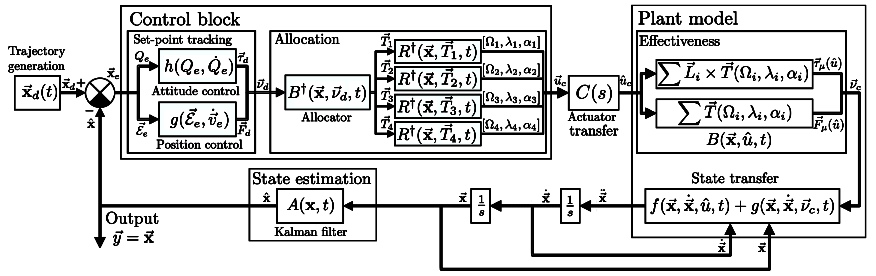
\includegraphics[width=0.63\textwidth]{figs/control-block}
\caption{Abstracted control block}
\label{fig:control-block}
\vspace{-15pt}
\end{figure}
\par
\emph{\color{Gray} Al allocation algorithms proposed follow the same input/output structure described in Fig:\ref{fig:control-block}. Only one allocation algorithm does, however, circumvent the virtual abstraction level of thrust vector's for each module to directly calculate actuator positions, Section:\ref{subsec:control.allocation.online}.}
\par
Each control law is co-dependent on an accompanying allocation algorithm. Traditional control loops (under-actuated or well matched) typically have a unity allocation rule and as such require no consideration so they're mostly disregarded. Separate control laws for attitude ad position control are presented next in Section:\ref{sec:control.attitude} and \ref{sec:control.position} respectively. Thereafter a series of allocation rules are proposed in Section:\ref{sec:control.allocation}. Although presented independently, the controller and allocation laws are mutually inclusive. The stability of each control law is proven objectively but actual controller tuning and optimization takes place only in the following Chapter:\ref{ch:simulation}, in Sec:\ref{sec:simulation.tuning}.
\par
%====================================================
\subsection*{Model Dependent \& Independent Controllers}
%====================================================
Two classes of controllers are presented, attitude and position control laws. The former being the primary focus of this research project and containing a more complete schedule of control treatment and controller comparison. Both control categories consider MIMO state vector loops for attitude and position states $\mathcal{E}$ \& $Q_b$. The allocation algorithm combines both virtual control inputs $\vec{\nu}_d=[\mu\vec{F}~\mu\vec{\tau}]^T$ generated from the two control categories to calculate actuator positions.
\par
The control dependency on the system plant is as a consequence of the prominent actuator response dynamics, as derived previously in Sec:\ref{subsec:dynamics.nonlinearities.gyrotorques}. Whilst not a prerequisite for stability, plant dependent compensation certainly improves controller performances. Independent and dependent cases are only considered for one type of controller; the most basic case PD controller in Section:\ref{subsec:control.attitude.controllers}. It's shown that for an independent (\emph{PD}) controller to achieve global stability some stringent assumptions must first be met.
\par
Inherent plant dependency makes backstepping controllers an attractive control paradigm in this dissertation's context. The proposed plant dependent control laws compensate for undesirable dynamics their design, basic PD \& PID control structures (\emph{and the like}) will not. The first and most basic control solution, used as a reference case, is a PD controller for attitude and position with direct-inversion\footnote{Pseudo-inversion or Moore-Penrose inversion} allocation, both plant dependent and independent PD controllers are compared.
%====================================================
\section{Lyapunov Stability Theorem}
\label{sec:control.lyapunov}
%====================================================
Lyapunov's stability theory is a critical aspect of non-linear controller design. An abundance of literature has been written on the subject\footnote{Included in almost every meritable textbook and papers; \cite{noteonlyapunov,nonlinearsystems}, amongst others\ldots} spanning through the progression of control engineering. Typically linear systems are proven$^\dagger$ to be stable using the frequency domain with Laplace transforms, the same is not true for non-linear systems. Lyapunov's stability theorem proves (\emph{global}) asymptotic stability for continuous time invariant systems, linear or otherwise.
\par
The theorem applies analysis of a generalized energy function representative of a system's autonomous trajectory. A negative trajectory energy derivative will ensure the system's energy is always dissipating toward a stable settling point. Lyapunov analysis is a popular method for stability verification because system's trajectory itself needn't be explicitly defined for stability to be ascertained. Proof of Lyapunov's theorem is done with a contradiction disproof and, as such, the theoretical underpinning is somewhat cumbersome.
\par
Despite the conceptually difficult proof, it's worth reiterating its fundamentals given that backstepping controllers are proposed later in Sec:\ref{subsec:control.attitude.nonlinear} for attitude control. A backstepping controller iteratively enforces Lyapunov stability criterion onto the system through the control structure. In general, given a non-linear time invariant system that follows some continually differentiable trajectory $\mathbf{x}(t)$, typically the trajectory is going to progress subject to some rule:
\begin{equation}
\dot{\mathbf{x}}(t)=f\big(\mathbf{x}(t)\big)
\end{equation}
Then, constructing a generalized positive-definite function (generalized energy or \emph{Lyapunov candidate} function) $V(x)$ for a trajectory $x=\mathbf{x}(t)$. A positive definite matrix, $M$, is defined such that $z^TMz\geq 0~\forall z$. As such an LCF typically has the form:
\begin{equation}
V=x^TPx
\end{equation}
Given that, by its definition, the trajectory is continually differentiable; there is a partial gradient matrix for each component of $V(x)$ in the form:
\begin{equation}
\nabla V(x)=\bigg[\frac{\delta V(x)}{\delta x_1}~\frac{\delta V(x)}{\delta x_2}~\ldots~\frac{\delta V(x)}{\delta x_n}\bigg]~~~~x\in\mathbb{R}^n
\end{equation}
The energy function's derivative, otherwise referred to as the \emph{Lie derivative}$^\dagger$, is calculated as follows:
\begin{equation}
\dot{V}(x)=\nabla V(x)^Tf(x)=\frac{\delta V(x)}{\delta x_1}f_1(x)+\frac{\delta V(x)}{\delta x_2}f_2(x_2)+~\ldots~+\frac{\delta V(x)}{\delta x_n}f_n(x)
\end{equation}
Lyapunov's theorem states that \emph{iff} the candidate function $V(x)$ is positive definite with $\dot{V}(0)=0$ and its derivative is negative definite; $\dot{V}(x)< 0~~\forall x \not= 0$, the system is then globally asymptotically stable. Mathematically that means, for any $\mathbf{x}(t)\geq 0$:
\begin{equation}
V\big(\mathbf{x}(t)\big)=V\big(\mathbf{x}(0)\big)+\int_0^t \dot{V}\big(\mathbf{x}(t)\big).dt \leq V\big(\mathbf{x}(t)\big)
\end{equation}
Which can be physically interpreted as the system's generalized energy function always dissipating, irrespective of trajectory path taken. With a continually decreasing energy function, the system will inevitably settle to some stable point, hence the trajectory exists in some bounded $\big\{x|V(x)\leq V\big(\mathbf{x}(t)\big)\big\}$, which is defined as global asymptotic stability. Every trajectory of $\dot{\mathbf{x}}(t)=f\big(\mathbf{x}(t)\big)$ converges to the zero\footnote{Adapted to zero error state tracking in lieu or zero set point settling.} setpoint as $t\rightarrow\infty$.
\par
The asymptotic stability proof can be extended to exponential stability boundedness, such that \emph{iff} the same conditions are met and there exists some positive coefficient $\alpha>0$ such that $\dot{V}(x)\leq-\alpha V(x)$. That implies the system is globally exponentially stable as is bound in such a way that:
\begin{equation}
\norm{\mathbf{x}(t)}\leq Me^{-\alpha t/2}\norm{\mathbf{x}(0)}
\end{equation}
%====================================================
\section{Attitude Control}
\label{sec:control.attitude}
%====================================================
\subsection{The Attitude Control Problem}
\label{subsec:control.attitude.problem}
%====================================================
Set point tracking control of the attitude plant is to then design a stabilizing control torque $\mu\vec{\tau}=h(\mathbf{x}_e,t)$ such that; for any desired attitude quaternion, $\forall~Q_d\in\mathbb{Q}$, and an instantaneous attitude body quaternion, similarly $\forall~Q_b\in\mathbb{Q}$, the error state asymptotically stabilizes to 0; $Q_e\rightarrow[1~\vec{0}~]^T$. Or that:
\begin{equation}
\mu\vec{\tau}=h(Q_e,~\dot{Q}_e)~~\text{such that}~~\underset{t\rightarrow\infty}{\lim}Q_e=\begin{bmatrix}
1\\
\vec{0}
\end{bmatrix}
\end{equation}
Quaternion error states are defined as the Hamilton product (\emph{difference}) between the desired and instantaneous quaternion attitude states. Quaternion error states are in contrast with the subtractive relationship for Euler angle error states. The attitude error state is calculated as:
\begin{equation}\label{eq:quaternion-error}
Q_e=Q_d^*\otimes Q_b
\end{equation}
The relative angular velocity error between the body frame, $\mathcal{F}^b$, and the trajectory's desired frame, $\mathcal{F}^d$, is given as $\vec{\omega}_e$. The body angular velocity, $\vec{\omega}_b$ is subject to the differential Eq:\ref{eq:quaternion-states-angular}. As such there's an angular rate error:
\begin{subequations}
\begin{equation}\label{eq:angular-error}
\vec{\omega}_e=\vec{\omega}_d-\vec{\omega}_b
\end{equation}
The desired angular rate is taken with respect to the desired angular attitude frame, and so it must be transformed back onto the existing body frame.
\begin{equation}
\vec{\omega}_e=Q_e^*\otimes\vec{\omega}_d\otimes Q_e-\vec{\omega}_b
\end{equation}
Typically for the trajectories generated here the desired angular velocity is zero; $\vec{\omega}_d=\vec{0}$. IT follows that the angular rate error is then simply the negative body angular velocity. It would be easy to incorporate a non-zero angular velocity setpoint to accommodate for higher order state derivative tracking trajectories.
\begin{equation}
\vec{\omega}_e=-\vec{\omega}_b\Big|_{\vec{\omega}_d=\vec{0}}
\end{equation}
\end{subequations}
The time derivative of the quaternion error state is given by Eq:\ref{eq:quaternion-deriv}. The derivative $\dot{Q}_e$ is then dependent on the angular velocity error and calculated as follows:
\begin{equation}
\dot{Q}_e=\frac{1}{2}Q_e\otimes\vec{\omega}_e=-\frac{1}{2}Q_e\otimes\vec{\omega}_b\Big|_{\vec{\omega}_d=\vec{0}}
\end{equation}
%====================================================
\subsection{Linear Controllers}
\label{subsec:control.attitude.controllers}
%====================================================
\subsubsection{PD Controller}
\label{subsubsec:control.attitude.controllers.pd}
%====================================================
The control law which is used as a basic reference for comparison is a simple Proportional-Derivative structured attitude controller. Specifically, a stability proof derived from the one presented \emph{The Attitude Control Problem}\cite{attitudecontrolproblem} is used for asymptotic stability verification. An attitude PD control law, proportional to the vector quaternion error only\footnote{Such that the error is $\in\mathbb{R}^3$.} and angular rate error, designs the control torque as:
\begin{equation}\label{eq:independent-pd}
\mu\vec{\tau}_{_{PD}}=K\vec{\omega}_e+\alpha\vec{q}_e
\end{equation}
Where both $K$ and $\alpha$ are positive definite symmetrical $3\times 3$ coefficient matrices still to be determined. This control law neglects the quaternion scalar error and is susceptible to unwinding. Then using a candidate Lyapunov energy function $V_{_{PD}}$:
\begin{equation}\label{eq:lyapunov-pd}
V_{_{PD}}(\vec{q}_e,\vec{\omega}_e)=\alpha\vec{q}_e\text{}^T\vec{q}_e+\alpha(q_0-1)^2+\frac{1}{2}\vec{\omega}_e\text{}^T\mathbb{I}_b\vec{\omega}_e
\end{equation}
And recalling from Eq:\ref{eq:quaternion-states-angular} that body's the angular velocity differential $\dot{\vec{\omega}}_b$ is:
\begin{equation}
\dot{\vec{\omega}}_b=\mathbb{I}_b\text{}^{-1}\big(-\vec{\omega}_b\times\mathbb{I}_b\vec{\omega}_b+\vec{\tau}_Q+\vec{\tau}_g+\vec{Q}+\mu\vec{\tau}\big)~~~~\in\mathcal{F}^b
\end{equation}
With actuator inputs $u\in\mathbb{U}$ implied and $\vec{Q}$ being a simplified representation of the net aerodynamic torque experienced by the body from the rotating propellers, drawn from Eq:\ref{eq:aerodynamic-torque}. Then, exploiting a unit quaternion's inherent property, it follows that:
\begin{equation}\label{eq:4.17}
\norm{Q}=\vec{q}\text{}^{\hspace{3pt}T}\vec{q}+q_0\text{}^2=\vec{q}\text{}^{\hspace{3pt}2}+q_0\text{}^2=1
\end{equation}
Substituting the angular velocity error state, $\vec{\omega}_e=-\vec{\omega}_b$, the proportional derivative LCF in Eq:\ref{eq:lyapunov-pd} is simplified\footnote{The quaternion scalar $q_0$ in Eq:\ref{eq:4.18} is implied to be the quaternion error state scalar} to:
\begin{subequations}\label{eq:4.18}
\begin{equation}
V_{_{PD}}=\alpha\vec{q}_e\text{}^2+\alpha q_0\text{}^2 -2q_0 + 1 +\frac{1}{2}\vec{\omega}_e\text{}^T\mathbb{I}_b\vec{\omega}_e
\end{equation}
\vspace{-10pt}
\begin{equation}
=2\alpha(1-q_0)+\frac{1}{2}\vec{\omega}_b\text{}^T\mathbb{I}_b\vec{\omega}_b
\end{equation}
\end{subequations}
Similarly, using the fact that for a quaternion's derivative:
\begin{equation}\label{eq:quat-derivative}
\dot{Q}=\begin{bmatrix}
-\frac{1}{2}\vec{q}^{\hspace{3pt}T}\vec{\omega}\\
\frac{1}{2}\big(\vec{q}_\times+q_0\mathbb{I}\big)\vec{\omega}
\end{bmatrix}
\end{equation}
Then, substituting the above into the derivative of the LCF, $\dot{V}_{_{PD}}$, yields:
\begin{subequations}
\begin{equation}
\dot{V}_{_{PD}}=2\alpha\frac{1}{2}\vec{q}_e\text{}^T\vec{\omega}_e+\frac{1}{2}\dot{\vec{\omega}}_b\text{}^T\mathbb{I}_b\vec{\omega}_b+\frac{1}{2}\vec{\omega}_b\mathbb{I}_b\dot{\vec{\omega}}_b\text{}^T
\end{equation}
\vspace{-12pt}
\begin{equation}
=-\alpha\vec{q}_e\text{}^T\vec{\omega}_b+\vec{\omega}_b\text{}^T\mathbb{I}_b\dot{\vec{\omega}}_b
\end{equation}
\end{subequations}
Simplifying the angular acceleration $\dot{\vec{\omega}}_b$ and introducing the PD control law Eq:\ref{eq:independent-pd}, $\mu\vec{\tau}_{_{PD}}$:
\begin{subequations}
\begin{equation}
\vec{\omega}_b\text{}^T\mathbb{I}_b\dot{\vec{\omega}}_b=\vec{\omega}_b\text{}^T\big(-\vec{\omega}_b\times\mathbb{I}_b\vec{\omega}_b+\vec{\tau}_Q+\vec{\tau}_g+\vec{Q}-K\vec{\omega}_b+\alpha\vec{q}_e\big)
\end{equation}
\vspace{-12pt}
\begin{equation}
\rightarrow\dot{V}_{_{PD}}=-\alpha\vec{q}_e\text{}^T\vec{\omega}_b+\vec{\omega}_b\text{}^T\big(-\vec{\omega}_b\times\mathbb{I}_b\vec{\omega}_b+\vec{\tau}_Q+\vec{\tau}_g+\vec{Q}-K\vec{\omega}_b+\alpha\vec{q}_e\big)
\end{equation}
\vspace{-10pt}
\begin{equation}
=-\alpha\vec{q}_e\text{}^T\vec{\omega}_b+\alpha\vec{\omega}_b\text{}^T\vec{q}_e-\vec{\omega}_b\text{}^TK\vec{\omega}_b+\vec{\omega}_b\text{}^T\big(-\vec{\omega}_b\times\mathbb{I}_b\vec{\omega}_b+\vec{\tau}_Q+\vec{\tau}_g+\vec{Q}\big)
\end{equation}
It follows that the transpose term $\vec{q}_e\text{}^T\vec{\omega}_b\iff\vec{\omega}_b\text{}^T\vec{q}_e$ is interchangeable as its resultant product is the same. The LCF derivative then simplifies to:
\begin{equation}
\dot{V}_{_{PD}}=-\vec{\omega}_b\text{}^TK\vec{\omega}_b+\vec{\omega}_b\text{}^T\big(-\vec{\omega}_b\times\mathbb{I}_b\vec{\omega}_b+\vec{\tau}_Q+\vec{\tau}_g+\vec{Q}\big)
\end{equation}
\end{subequations}
Then, under specific circumstances the following assumptions can be made to ensure the asymptotic stability proof can be applied. The stability obviously breaks down if any of the assumptions fail, as such the stability is not global\ldots
\vspace{-10pt}
\begin{enumerate}[itemsep=0em]
\item The inertial matrix, $\mathbb{I}_b$, is approximately diagonal. Which, given the symmetrical design and similarly that the angular rate can be made small with appropriately slow trajectory updates, is a fair assumption then:
\begin{center}
\vspace{-10pt}
$\vec{\omega}_b^{~T}\big(\vec{\omega}_b\times\mathbb{I}_b\vec{\omega}_b\big)\approx\vec{0}$
\vspace{-8pt}
\end{center}
\item The actuator rate torque responses, $\vec{\tau}_Q$, are all second order effects dependent on $\dot{u}$. Typically the actuator rates are going to be kept small and so any of the inertial responses to those position changes are small enough to be considered negligible. The approximation is made:
\begin{center}
\vspace{-10pt}
$\vec{\tau}_Q\approx\vec{0}$
\vspace{-8pt}
\end{center}
\item Finally, for the sake of the stability proof, the eccentric gravitational torque arm is neglected, $\vec{\tau}_g\approx\vec{0}$. Such a situation only holds true if $u\approx\vec{0}$ or that servo actuator positions\footnote{Excluding propeller rotational speeds, considering only the servo positions} are close to their zero positions.
\end{enumerate}
{\emph{\color{Gray}All of these assumptions are made under extraneous circumstances and can't be assumed for almost all of the prototype's flight envelope. The plant independent case is considered and simulated purely for contrition; mainly to demonstrate the need for plant dependent compensation. All subsequent control laws compensate for the plant dynamic response torques introduced in Section:\ref{sec:dynamics.nonlinearities}.}
\par
If each of the assumptions made hold true, then the Lyapunov energy function's derivative is approximately negative definite.
\begin{subequations}
\begin{equation}
\dot{V}_{_{PD}}\approx-\alpha\vec{q}_e\text{}^T\vec{\omega}_b+\vec{\omega}_b\text{}^T\big(-K\vec{\omega}_b+\alpha\vec{q}_e\big)
\end{equation}
\vspace{-10pt}
\begin{equation}
\Rightarrow\dot{V}_{_{PD}}=-\vec{\omega}_b\text{}^TK\vec{\omega}_b=-K\norm{\vec{\omega}_b}\text{}^2<\vec{0}~~~~\forall~(\vec{\omega}_e,Q_b)=\mathbf{z}(t)
\end{equation}
\end{subequations}
Where $\mathbf{z}(t)$ is a generalized attitude trajectory which includes $\vec{\omega}_b$ \& $Q_b$ and K is a symmetrical\footnote{Symmetry, unlike the subsequent Auxiliary controller, is not a prerequisite for stability\ldots} positive (\emph{definite}) 3X3 coefficient matrix. Then from Lyapunov stability theorem the limits exist; $\lim_{t\rightarrow\infty}\vec{\omega}_e=\vec{0}$, $\lim_{t\rightarrow\infty}\vec{q}_e=0$ and $\lim_{t\rightarrow\infty}(1-q_0)=0$. Hence $Q_e\rightarrow[1~\vec{0}\hspace{3pt}]^{T}$ as $t\rightarrow\infty$, asymptotically stabilizing the attitude error state. 
\par
Introducing model dependent compensation to the PD control law in Eq:\ref{eq:independent-pd} alleviates the stringent requirements on assumptions 1 through 3. 
\begin{equation}\label{eq:dependent-pd}
\mu\vec{\tau}_{_{PD}}=\vec{\omega}_b\times\mathbb{I}_b\vec{\omega}_b-\vec{\tau}_Q-\vec{\tau}_g-\vec{Q}+K\vec{\omega}_b+\alpha\vec{q}_e
\end{equation}
The resultant stability proof for Eq:\ref{eq:dependent-pd} is much the same as that for the independent case, Eq:\ref{eq:independent-pd}, and uses the identical LCF from Eq:\ref{eq:lyapunov-pd}. The resultant dependent control law is no longer reliant on the very broad assumptions needed for independent stability to be achieved. The dynamic compensation in Eq:\ref{eq:dependent-pd} improves control response, especially considering the form of unwanted dynamics which have already quantified previously and modelled with \emph{relative} confidence.
%====================================================
\subsubsection{Auxiliary Plant Controller}
\label{subsubsec:control.attitude.controllers.auxpd}
%====================================================
Expanding on what has, in practice\footnote{Practical examples of various quadrotor attitude PD controllers listed in Table:\ref{tab:controllers} from Sec:\ref{subsec:intro.lit.related}.}, proven to be a very popular and effective control law for attitude stabilization, McGilvray et al. [2006]\cite{attitudestabilization} suggested introducing an auxiliary plant term to a Proportional-Derivative structure. Most significantly, their altered PD controller adds auxiliary terms proportional to the quaternion time derivative error. The critical component of that change is the part of the auxiliary plant proportional to the quaternion scalar. The scalar term is otherwise neglected in the previous PD control law (Sec:\ref{subsubsec:control.attitude.controllers.pd}) and prevents unwinding if incorporated.
\par
The modified (\emph{auxilliarly}) PD control torque is a function of errors states for quaternions, angular rates and quaternion rates. The compensating plant dependent control law is given as:
\begin{equation}\label{eq:control-aux-pd}
\mu\vec{\tau}_{_{XPD}}=\underbrace{-\Gamma_2{\widetilde{\Omega}}-\Gamma_3\vec{q}_e+\mathbb{I}_b\dot{\bar{\Omega}}}_{Independent}+\underbrace{\vec{\omega}_b\times\mathbb{I}_b\vec{\omega}_b+\vec{\tau}_Q+\vec{\tau}_g+\vec{Q}}_{Compensation}
\end{equation}
In which case the coefficients\footnote{Reiterating that exact coefficient values are determined in Chapter:\ref{ch:simulation}\ldots} $\Gamma_2$ \& $\Gamma_3$ are both diagonal positive definite coefficient matrices and $\Gamma_1$, introduced subsequently in Eq:\ref{eq:aux-pd-2}, is a p.d symmetrical coefficient matrix. The auxiliary plants $\widetilde{\Omega}$ \& $\dot{\bar{\Omega}}$ are defined as follows and draw on Eq:\ref{eq:quat-derivative} for definition of some aspects. For the first auxiliary plant $\bar{\Omega}$ is proportional to the quaternion error and hence $\dot{\bar{\Omega}}$ is a quaternion derivative term:
\begin{subequations}\label{eq:aux-pd-1}
\begin{equation}
\bar{\Omega}=-\Gamma_1\vec{q}_e \Rightarrow\dot{\bar{\Omega}}=-\Gamma_1\dot{\vec{q}}_e
\end{equation}
\vspace{-15pt}
\begin{equation}
\dot{\bar{\Omega}}=-\frac{1}{2}\Gamma_1\big(q_0\mathbb{I}_{3X3}+[\vec{q}_e]_{\times}\big)\vec{\omega}_e
\end{equation}
\vspace{-10pt}
\begin{equation}
=\frac{1}{2}\Gamma_1\big(q_0\mathbb{I}_{3X3}+[\vec{q}_e]_{\times}\big)\vec{\omega}_b
\end{equation}
\end{subequations}
The second auxiliary plant, $\widetilde{\Omega}$, is a term proportional to a combined quaternion vector and angular velocity error state.
\begin{subequations}\label{eq:aux-pd-2}
\begin{equation}
\widetilde{\Omega}=\vec{\omega}_e-\bar{\Omega}=\vec{\omega}_e+\Gamma_1\vec{q}_e
\end{equation}
\vspace{-15pt}
\begin{equation}
=-\vec{\omega}_b+\Gamma_1\vec{q}_e
\end{equation}
\end{subequations}
Using an LCF similar to the basic one $V_{_{PD}}$ from Eq:\ref{eq:lyapunov-pd}, but introducing an auxiliary term $\widetilde{\Omega}$ into the candidate function $V_{_{XPD}}$:
\begin{equation}\label{eq:lyapunov-xpd}
V_{_{XPD}}\big(\vec{q}_e,~\widetilde{\Omega}\big)=\vec{q}_e\text{}^T\vec{q}_e+\big(q_0-1\big)^2+\frac{1}{2}\widetilde{\Omega}\text{}^{\hspace{1pt}T}\big(\Gamma_3^{-1}\mathbb{I}_b\big)\widetilde{\Omega}
\end{equation}
Again using the simplification from a quaternion's inherent properties in Eq:\ref{eq:4.17}, the LCF from Eq:\ref{eq:lyapunov-xpd} then simplifies with the following derivative:
\begin{subequations}
\vspace{-5pt}
\begin{equation}
V_{_{XPD}}=2(1-q_0)+\frac{1}{2}\widetilde{\Omega}\text{}^{\hspace{1pt}T}\big(\Gamma_3^{-1}\mathbb{I}_b\big)\widetilde{\Omega}
\end{equation}
\vspace{-10pt}
\begin{equation}
\dot{V}_{_{XPD}}=2\frac{1}{2}\vec{q}_e\text{}^T\vec{\omega}_e+\frac{1}{2}\dot{\widetilde{\Omega}}\text{}^{\hspace{1pt}T}\big(\Gamma_3^{-1}\mathbb{I}_b\big)\widetilde{\Omega}+\frac{1}{2}\widetilde{\Omega}\text{}^{\hspace{1pt}T}\big(\Gamma_3^{-1}\mathbb{I}_b\big)\dot{\widetilde{\Omega}}
\end{equation}
\vspace{-10pt}
\begin{equation}\label{eq:4.34c}
\dot{V}_{_{XPD}}=-\vec{q}_e\text{}^T\vec{\omega}_b+\frac{1}{2}\dot{\widetilde{\Omega}}\text{}^{\hspace{1pt}T}\big(\Gamma_3^{-1}\mathbb{I}_b\big)\widetilde{\Omega}+\frac{1}{2}\widetilde{\Omega}\text{}^{\hspace{1pt}T}\big(\Gamma_3^{-1}\mathbb{I}_b\big)\dot{\widetilde{\Omega}}
\end{equation}
\end{subequations}
It follows that from Eq:\ref{eq:aux-pd-2} then the auxiliary plant derivative $\dot{\widetilde{\Omega}}$ is:
\begin{subequations}
\begin{equation}
\dot{\widetilde{\Omega}}=-\dot{\vec{\omega}}_b+\Gamma_1\dot{\bar{\Omega}}\Rightarrow\dot{\vec{\omega}}_b=\mathbb{I}_b^{-1}\big(-\vec{\omega}_b\times\mathbb{I}_b\vec{\omega}_b+\vec{\tau}_Q+\vec{\tau}_g+\vec{Q}+\mu\vec{\tau}\big)
\end{equation}
\vspace{-15pt}
\begin{equation}
\therefore\dot{\widetilde{\Omega}}=-\mathbb{I}_b^{-1}\big(-\vec{\omega}_b\times\mathbb{I}_b\vec{\omega}_b+\vec{\tau}_Q+\vec{\tau}_g+\vec{Q}+\mu\vec{\tau}\big)-\Gamma_1\dot{\bar{\Omega}}
\end{equation}
Substituting the auxiliary PD control law, $\mu\vec{\tau}_{_{XPD}}$ from Eq:\ref{eq:control-aux-pd}, into the auxiliary plant derivative then yields:
\begin{equation}
\rightarrow\dot{\widetilde{\Omega}}=\mathbb{I}_b^{-1}\big(\mathbb{I}_b\dot{\bar{\Omega}}-\Gamma_2\widetilde{\Omega}-\Gamma_3\vec{q}_e\big)-\dot{\bar{\Omega}}
\end{equation}
\vspace{-15pt}
\begin{equation}
=\mathbb{I}_b^{-1}\big(-\Gamma_2\widetilde{\Omega}-\Gamma_3\vec{q}_e\big)
\end{equation}
\end{subequations}
From the positive symmetric (or \emph{diagonal}) properties of the coefficient matrices $\Gamma_1$,$\Gamma_2$ \& $\Gamma_3$, the auxiliary plant's transpose is then:
\begin{equation}
\dot{\widetilde{\Omega}}\text{}^{\hspace{1pt}T}=\mathbb{I}_b^{-1}\big(-\Gamma_2\widetilde{\Omega}^{\hspace{1pt}T}-\Gamma_3\vec{q}_e\text{}^T\big)
\end{equation}
It then follows that the P.D auxiliary plant component in the LCF, Eq:\ref{eq:lyapunov-xpd}, simplifies:
\begin{subequations}
\begin{equation}
\frac{1}{2}\dot{\widetilde{\Omega}}\text{}^{\hspace{1pt}T}\big(\Gamma_3^{-1}\mathbb{I}_b\big)\widetilde{\Omega}=\frac{1}{2}\big(-\Gamma_2\widetilde{\Omega}\text{}^{\hspace{1pt}T}-\Gamma_3\vec{q}_e\text{}^T\big)\Gamma_3^{-1}\widetilde{\Omega}
\end{equation}
\vspace{-10pt}
\begin{equation}
=\frac{1}{2}\big(-\widetilde{\Omega}\text{}^{\hspace{1pt}T}\Gamma_2\Gamma_3^{-1}\widetilde{\Omega}-\vec{q}_e\text{}^{T}\widetilde{\Omega}\big)
\end{equation}
And substituting Eq:\ref{eq:aux-pd-2}, $\vec{q}_e\text{}^T\widetilde{\Omega}=-\vec{q}_e\text{}^T\vec{\omega}_b+\Gamma_1\vec{q}_e\text{}^T$:
\begin{equation}
\frac{1}{2}\big(-\widetilde{\Omega}\text{}^{\hspace{1pt}T}\Gamma_2\Gamma_3^{-1}\widetilde{\Omega}+\vec{q}_e\text{}^T\vec{\omega}_b-\vec{q}_e\text{}^T\Gamma_1\vec{q}_e\big)
\end{equation}
Similarly, for the transposed energy function counterpart:
\begin{equation}
\frac{1}{2}\widetilde{\Omega}\text{}^{\hspace{1pt}T}\big(\Gamma_3^{-1}\mathbb{I}_b\big)\dot{\widetilde{\Omega}}=\frac{1}{2}\big(-\widetilde{\Omega}\Gamma_2\Gamma_3^{-1}\widetilde{\Omega}\text{}^{\hspace{1pt}T}+\vec{q}_e\text{}^T\vec{\omega}_b-\vec{q}_e\Gamma_1\vec{q}_e\text{}^T\big)
\end{equation}
Which, when substituted back into Eq:\ref{eq:4.34c}, then simplifies the LCF derivative to negative definite:
\end{subequations}
\begin{equation}
\Rightarrow\dot{V}_{_{XPD}}=-\vec{q}_e\text{}^T\Gamma_1\vec{q}_e-\widetilde{\Omega}\Gamma_2\Gamma_3^{-1}\widetilde{\Omega}\text{}^{\hspace{1pt}T}<\vec{0}~~~~\forall~(\vec{q}_e,\widetilde{\Omega})
\end{equation}
As such, the control law $\mu\vec{\tau}_{_{XPD}}$ asymptomatically stabilizes the attitude plant. Both $\widetilde{\Omega}$ and $\vec{q}_e$ tend to $\vec{0}$, or more specifically the following limits exist:
\begin{subequations}
\begin{equation}
\underset{t\rightarrow\infty}{\lim}\vec{q}_e=0~~\text{and}~~\underset{t\rightarrow\infty}{\lim}\widetilde{\Omega}=0
\end{equation}
Then, from the auxiliary plant definition in Eq:\ref{eq:aux-pd-2}, the extended limits present themselves;
\begin{equation}
\underset{t\rightarrow\infty}{\lim}\vec{\omega}_b=0~~~\text{and}~~~\underset{t\rightarrow\infty}{\lim}\bar{\Omega}=0
\end{equation}
\end{subequations}
\par
The stability proof for $V_{_{XPD}}$ can then be extended to a stable exponentially bounded trajectory. From a quaternion's inherent definition it follows that $0\leq q_0 \leq 1$. It can then be stated that:
\begin{equation}\label{eq:4.34}
1-q_0\leq 1-q_0^2=\norm{\vec{q}_e}^2
\end{equation}
Seeing that exponential stability is a maximal boundedness proof, the relationship Eq:\ref{eq:4.34} can then replace the quaternion scalar term $2(1-q_e)$ in $V_{_{XPD}}$. For the stability proof the LCF is rewritten in terms of its component's norm(s) to produce the inequality:
\begin{subequations}\label{eq:xpd-ibc}
\begin{equation}
V_{_{XPD}}=\vec{q}_e\text{}^T\vec{q}_e+(q_0-1)^2+\frac{1}{2}\widetilde{\Omega}\text{}^{\hspace{1pt}T}\big(\Gamma_3^{-1}\mathbb{I}_b\big)\widetilde{\Omega}
\end{equation}
\vspace{-10pt}
\begin{equation}
\rightarrow V_{_{XPD}}\leq 2\norm{\vec{q}_e}\text{}^2+\frac{1}{2}\Gamma_3^{-1}\mathbb{I}_b||\widetilde{\Omega}||\text{}^2
\end{equation}
Similarly the LCF derivative can be written in terms of its norms as:
\begin{equation}
\dot{V}_{_{XPD}}=-\Gamma_2\Gamma_3^{-1}||\widetilde{\Omega}||\text{}^2-\Gamma_1\norm{\vec{q}_e}\text{}^2
\end{equation}
\end{subequations}
$V_{_{XPD}}$ then gains a maximum such that:
\begin{equation}
V_{_{XPD}}\leq max \bigg\{ 2,\frac{\lambda_{max}(\Gamma_3^{-1}\mathbb{I}_b)}{2}\bigg\}\big(\norm{\vec{q}_e}\text{}^2+||\widetilde{\Omega}||\text{}^2\big)
\end{equation}
Where the function $\lambda_{max}$ represents the maximum eigenvalue of its argument, in this case $\Gamma_3^{-1}\mathbb{I}_b$. Similarly the \emph{negative definite} LCF derivative is bound by the minimum:
\begin{equation}
\dot{V}_{_{XPD}} \leq -min \big\{ \lambda_{min}(\Gamma_1),\lambda_{min}(\Gamma_2\Gamma_3\text{}^{-1})\big\}\big(\norm{\vec{q}_e}\text{}^2+||\widetilde{\Omega}||^2 \big)
\end{equation}
Therefore there exists some ratio $\alpha>0$ that satisfies the relationship requirement between the LCF and its derivative; $\dot{V}_{_{XPD}}\leq -\alpha V_{_{XPD}}$, where $\alpha$ is defined as the ratio of those maxima\footnote{A maximum and minimum}:
\begin{equation}
\alpha=\frac{min\big\{\lambda_{min}(\Gamma_1),\lambda_{min}(\Gamma_2\Gamma_3\text{}^{-1})\big\}}{max\big\{2,\frac{\lambda_{max}(\Gamma_3\text{}^{-1}\mathbb{I}_b)}{2}\big\}}
\end{equation}
The attitude trajectory $\big(\vec{q}_e(t),\widetilde{\Omega}(t)\big)$ is then exponentially bounded by:
\begin{equation}
\big(\norm{\vec{q}_e(t)},||\widetilde{\Omega}(t)||\big)\leq Me^{-\alpha t/2}\big(\norm{\vec{q}_e(0)},||\widetilde{\Omega}(0)||\big)
\end{equation}
\par
\vspace{-10pt}
\emph{\color{Gray}The above stability proof for the auxiliary attitude controller was expanded upon and derived from McGilvray et al. [2006]\cite{attitudestabilization} and adapted to fit attitude setpoint tracking. The fact that the auxiliary plant controller introduces the quaternion error, which is dependent on the quaternion scalar, dramatically improves controller performance. The exponential stability notably improves settling times and overshoot errors, seen next in Chapter:\ref{ch:simulation}.}
\par
Interestingly an earlier paper by Joshi, et al. [1995]\cite{robustattitude} was the precursor for PD based attitude plants with asymptotic exponential stability. Joshi's control law first proposed didn't make use of any defined auxiliary plants, unlike \cite{attitudestabilization}, but equivalent terms were effectively incorporated. That control law developed for spacecraft attitude tracking proposed a very similar exponentially stabilizing control scheme to that of $\mu\vec{\tau}_{_{XPD}}$. That controller, when changed to the notational convention used above, designs body torque as:
\begin{equation}
\mu\vec{\tau}^{\hspace{3pt}'}_{_{XPD}}=-\frac{1}{2}\Big[\big([\vec{q}_e]_\times+q_0\mathbb{I}_{3X3}\big)\Gamma_1+\alpha\big(1-q_0\mathbb{I}\big)\Big]\vec{q}_e-\Gamma_2\vec{\omega}_b
\end{equation} 
%====================================================
\subsection{Non-linear Controllers}
\label{subsec:control.attitude.nonlinear}
%====================================================
Backstepping controllers(presented in \cite{satellitebackstepping,intelligentbackstep,backstepslidingmode},etc\ldots) are a popular choice for non-linear attitude control plants. The process, through iterative design, enforces Lyapunov stability criteria to ensure asymptotic stability. In a report \cite{backstepping} Van Kampen, et al. [2008] describes fundamental backstepping algorithms. Ideal backstepping control is a precise control solution which requires exact plant matching, something that is difficult to achieve in practice. Another caveat of IBC control is poor disturbance rejection, being especially susceptible to plant uncertainty. The ideal backstepping algorithm can then be extended to incorporate non-idealities. The disturbance and uncertainty (\emph{estimate error}) terms are incorporated into the LCF energy function. By Lyapunov's theorem their respective estimation error terms are stabilized.
%====================================================
\subsubsection{Ideal Backstepping Controller}
\label{subsubsec:control.attitude.nonlinear.idealbackstep}
%====================================================
Starting with the ideal case for the first proposed backstepping controller; it's assumed the attitude plant described in Eq:\ref{eq:quaternion-states-angular}, from the consolidated model in Sec:\ref{sec:dynamics.model}, absolutely matches the dynamics of the physical prototype. The ideal backstepping controller aims to perfectly compensate for the plant's dynamic response to trajectory inputs. Ignoring any uncertainty associated with the dynamic equation, the aim here is to apply a stabilizing torque design. Recalling the quaternion tracking error from Eq:\ref{eq:quaternion-error}; $Q_e=Q_d^*\otimes Q_b$. Then considering the first LCF proposal:
\begin{equation}
V_1(\vec{q}_e)=\vec{q}_e\text{}^T\vec{q}_e+(q_0-1)^2
\end{equation}
Which, after substituting in the quaternion derivatives and \emph{without} using the quaternion simplification in Eq:\ref{eq:4.18}, has a Lie derivative:
\begin{subequations}
\begin{equation}
\dot{V}_1=2\vec{q}_e\text{}^T\dot{\vec{q}}_e+2(q_0-1)\dot{q}_0
\end{equation}
\vspace{-10pt}
\begin{equation}
=2\vec{q}_e\text{}^T\frac{1}{2}\big([\vec{q}_e]_\times+q_0\mathbb{I}_{3X3}\big)\vec{\omega}_e-2\big(q_0-1\big)\frac{1}{2}\vec{q}_e\text{}^T\vec{\omega}_e
\end{equation}
\vspace{-5pt}
\begin{equation}
=\vec{q}_e\text{}^T\big([\vec{q}_e]_\times+q_0\mathbb{I}_{3X3}\big)\vec{\omega}_e-q_0\vec{q}_e\text{}^T\vec{\omega}_e+\vec{q}_e\text{}^T\vec{\omega}_e
\end{equation}
\vspace{-10pt}
\begin{equation}
=\vec{q}_e\text{}^T[\vec{q}_e]_\times\vec{\omega}_e+\vec{q}_e\text{}^T\vec{\omega}_e
\end{equation}
\vspace{-10pt}
\begin{equation}
=-\vec{q}_e\text{}^T[\vec{q}_e]_\times\vec{\omega}_b-\vec{q}_e\text{}^T\vec{\omega}_b
\end{equation}
\end{subequations}
Then choosing the first stabilizing function, $z_1$, with a virtual backstepping control input $\Omega_d$. It's important to note that $\Omega_d$ is used here to differentiate the backstepping \emph{desired} value from the trajectory instructed $\vec{\omega}_d$ from Eq:\ref{eq:angular-error}, or any auxiliary plants defined previously for the Auxiliary PD controller in Sec:\ref{subsubsec:control.attitude.controllers.auxpd}.
\begin{equation}
\vec{\omega}_b\Rightarrow\Omega_d=\Gamma_1\vec{q}_e
\end{equation}
Where $\Gamma_1$ is the first symmetric positive definite coefficient matrix, a fact that is important to stress due to positive definite matrix's invertability. That stabilizing law then simplifies the LCF derivative $\dot{V}_1$ to the negative definite term:
\begin{subequations}
\begin{equation}
\dot{V}_1=-\vec{q}_e\text{}^T[\vec{q}_e]_\times\Omega_d-\vec{q}_e\text{}^T\Omega_d
\end{equation}
\vspace{-14pt}
\begin{equation}
=-\vec{q}_e\text{}^T[\vec{q}_e]_\times\Gamma_1\vec{q}_e-\vec{q}_e\text{}^T\Gamma_1\vec{q}_e
\end{equation}
\vspace{-12pt}
\begin{equation}
=-\vec{q}_e\text{}^T\Gamma_1\vec{q}_e
\end{equation}
\end{subequations}
A vector cross product with itself has a zero resultant. However, that stabilizing virtual plant input $\Omega_d$ has its own associated error, $z_1$, which then needs to be stabilized as well:
\begin{subequations}
\begin{equation}
z_1=\vec{\omega}_b-\Omega_d=\vec{\omega}_b-\Gamma_1\vec{q}_e
\end{equation}
\vspace{-15pt}
\begin{equation}
\rightarrow \vec{\omega}_b=z_1-\Gamma_1\vec{q}_e
\end{equation}
\end{subequations}
Introducing that error $z_1$ into a second LCF, which expands the first proposed $V_1$. Here is where it's important that $\Gamma_1$ is p.d \& symmetrical:
\begin{subequations}
\begin{equation}
V_2(\vec{q}_e,z_1)=V_1(\vec{q}_e)+\frac{1}{2}z_1\text{}^T\Gamma_1^{-1}z_1
\end{equation}
\vspace{-10pt}
\begin{equation}
=\vec{q}_e\text{}^T\vec{q}_e+(q_0-1)^2+\frac{1}{2}z_1\text{}^T\Gamma_1^{-1}z_1
\end{equation}
\end{subequations}
That first error $z_1$ has its own derivative, and recalling $\dot{\vec{\omega}}_b$ from earlier with an as yet undefined controllable input $\mu\vec{\tau}$, which still has plant dependency compensation.
\begin{subequations}
\begin{equation}
\dot{z}_1=\dot{\vec{\omega}}_b-\Gamma_1\dot{\vec{q}}_e
\end{equation}
\vspace{-10pt}
\begin{equation}
=\dot{\vec{\omega}}_b-\frac{\Gamma_1}{2}\big([\vec{q}_e]_\times+q_0\mathbb{I}_{3X3}\big)\vec{\omega}_e
\end{equation}
\vspace{-10pt}
\begin{equation}\label{eq:z-deriv}
=\mathbb{I}_b^{-1}\big(-\vec{\omega}_b\times\mathbb{I}_b\vec{\omega}_b+\vec{\tau}_Q+\vec{\tau}_g+\vec{Q}+\mu\vec{\tau}\big)+\frac{\Gamma_1}{2}\big([\vec{q}_e]_\times+q_0\mathbb{I}_{3X3}\big)\vec{\omega}_b
\end{equation}
\end{subequations}
So then, following from Eq:\ref{eq:z-deriv}, finding the derivative $\dot{V}_2$:
\begin{subequations}\label{eq:ibc-deriv}
\begin{multline}
\dot{V}_2(\vec{q}_e,~z_1)=\vec{q}_e\text{}^T\big(z_1-\Gamma_1\vec{q}_e\big)+z_1\text{}^T\Gamma_1^{-1}\bigg(\mathbb{I}_b^{-1}\big(-\vec{\omega}_b\times\mathbb{I}_b\vec{\omega}_b+\vec{\tau}_Q+\vec{\tau}_g+\vec{Q}+\mu\vec{\tau}\big)\\+\frac{\Gamma_1}{2}\big([\vec{q}_e]_\times+q_0\mathbb{I}_{3X3}\big)\vec{\omega}_b\bigg)
\end{multline}
\vspace{-20pt}
\begin{multline}
=-\vec{q}_e\text{}^T\Gamma_1\vec{q}_e+z_1\text{}^T\Gamma_1^{-1}\bigg(\Gamma_1\vec{q}_e+\mathbb{I}_b^{-1}\big(\vec{\omega}_b\times\mathbb{I}_b\vec{\omega}_b+\vec{\tau}_Q+\vec{\tau}_g+\vec{Q}+\mu\vec{\tau}\big)\\+\frac{\Gamma_1}{2}\big([\vec{q}_e]_\times+q_0\mathbb{I}_{3X3}\big)\vec{\omega}_b\bigg)
\end{multline}
\end{subequations}
Then proposing the compensated stabilizing backstepping control law:
\begin{equation}\label{eq:control-ibc}
\mu\vec{\tau}_{_{IBC}}=\vec{\omega}_b\times\mathbb{I}_b\vec{\omega}_b-\vec{\tau}_Q-\vec{\tau}_g-\vec{Q}-\mathbb{I}_b\Gamma_1\vec{q}_e-\frac{\mathbb{I}_b\Gamma_1}{2}\big([\vec{q}_e]_\times+q_0\mathbb{I}_{3X3}\big)\vec{\omega}_b-\mathbb{I}_b\Gamma_2z_1
\end{equation}
With $\Gamma_2$ being another positive definite symmetric coefficient matrix. Then with the control law $\mu\vec{\tau}_{_{IBC}}$ introduced into the LCF derivative $\dot{V}_2$ simplifies to negative definite:
\begin{equation}
\dot{V}_2=-\vec{q}_e\text{}^T\Gamma_1\vec{q}_e-z_1\text{}^T\Gamma_2z_1\leq \vec{0}~~~~\forall~(\vec{q}_e,z_1)
\end{equation}
As such $\vec{q}_e\rightarrow 0$ \& $q_0\rightarrow 1$ as $t\rightarrow\infty$. Similarly $z_1\rightarrow 0$, which leads to the limit:
\begin{equation}
\underset{t\rightarrow\infty}{\lim}(\vec{\omega}_b-\Gamma_1\vec{q}_e)=0
\end{equation} 
Because the quaternion error vector already tends to $0$; $\vec{q}_e\rightarrow 0$, it follows that $\vec{\omega}_b\rightarrow 0$. It can also be said that, from the definition of $\vec{\omega}_e$, that the angular velocity error stabilizes too. There is a distinct similarity in the structure of $\mu\vec{\tau}_{_{IBC}}$ from Eq:\ref{eq:control-ibc} and that of the auxiliary PD controller presented in Eq:\ref{eq:control-aux-pd}. Furthermore, using the same reasoning from Eq:\ref{eq:xpd-ibc}, the exponential stability proof then follows:
\begin{subequations}
\begin{equation}
V_{_{IBC}}\leq V_2=2\norm{\vec{q}_e}\text{}^2+\frac{\Gamma_1^{-1}}{2}\norm{z_1}\text{}^2
\end{equation}
\vspace{-15pt}
\begin{equation}
\dot{V}_{_{IBC}}\leq\dot{V}_2=-\Gamma_1\norm{\vec{q}_e}\text{}^2-\Gamma_2\norm{z_1}\text{}^2
\end{equation}
\end{subequations}
Then both the energy function and its derivative are bound respectively by:
\begin{subequations}
\begin{equation}
V_{_{IBC}}\leq max\bigg\{2,~\frac{\lambda_{max}(\Gamma_1\text{}^{-1})}{2}\bigg\}(\norm{\vec{q}_e}\text{}^2+\norm{z_1}\text{}^2)
\end{equation}
\vspace{-10pt}
\begin{equation}
\dot{V}_{_{IBC}}\leq min\big\{\lambda_{min}(\Gamma_1),~\lambda_{min}(\Gamma_2)\big\}(\norm{\vec{q}_e}\text{}^2+\norm{z_1}\text{}^2)
\end{equation}
\end{subequations}
Which then leads to a similar exponential stability trajectory boundedness such that:
\begin{subequations}
\begin{equation}
\dot{V}_{_{IBC}} \leq \alpha V_{_{IBC}}
\end{equation}
\vspace{-15pt}
\begin{equation}
\therefore \big(\norm{\vec{q}_e(t)},\norm{z_1(t)}\big)\leq Me^{-\alpha t/2}\big(\norm{\vec{q}_e(0)},\norm{z_1(0)}\big)
\end{equation}
\end{subequations}
%====================================================
\subsubsection{Adaptive Backstepping Controller}
\label{subsubsec:control.attitude.nonlinear.adaptivebackstep}
%====================================================
As effective as the control law defined above in Section:\ref{subsubsec:control.attitude.nonlinear.idealbackstep} may be, it lacks suitable disturbance rejection properties. Any plant uncertainties or disturbances encountered would adversely affect the controller in a dramatic manner (Sec:\ref{sec:simulation.comparison}). Introducing a term for lumped uncertainty/disturbance torques, $\vec{L}$, into the dynamic equations leads to:
\begin{equation}
\dot{\vec{\omega}}_b=\mathbb{I}_b\text{}^{-1}\big(-\vec{\omega}_b\times\mathbb{I}_b\vec{\omega}_b+\vec{\tau}_Q+\vec{\tau}_g+\vec{Q}+\vec{L}+\mu\vec{\tau}\big)
\end{equation}
It would obviously be easy to simply introduce a compensation term for $-\vec{L}$ into the control law. In practice, however, it is very difficult to approximate a disturbance term without \emph{apriori} knowledge about any of its properties. Noise compensation in sensors can be done easily due to the known frequency bandwidth which that noise occurs in, the same cannot be said for wind disturbances and the like.
\par
An approximate estimation term $\hat{L}$ has to be used for that disturbance compensation in the designed control torque $\mu\vec{\tau}$. That estimate term is then going to have its own error from the physical disturbance affecting the system:
\begin{equation}\label{eq:estimate-error}
\widetilde{L}=\vec{L}-\hat{L}
\end{equation}
The purpose of adaptive backstepping is to introduce that estimate error term into an LCF and develop a derivative term for $\dot{\hat{L}}$, or a disturbance update law, such that even the estimate error asymptotically stabilizes. Typically, that disturbance update rule is the contribution of satellite and general attitude control papers. Similar terms can be introduced for plant uncertainty which can similarly be adapted for but are not included here\ldots
\par
The estimate error is then introduced into the LCF from an ideal backstepping control, in order for it to be dissipated as per Lyapunov theorem.
\begin{subequations}
\begin{equation}
V_{_{ABC}}(\vec{q}_e,z_1,\widetilde{L})=V_{_{IBC}}(\vec{q}_e,z_1)+\frac{1}{2}\widetilde{L}\text{}^T \Gamma_L^{-1}\widetilde{L}
\end{equation}
\vspace{-10pt}
\begin{equation}
=\vec{q}_e\text{}^T\vec{q}_e+(q_0-1)^2+\frac{1}{2}z_1\text{}^T\Gamma_1^{-1}z_1+\frac{1}{2}\widetilde{L}\text{}^T\Gamma_L^{-1}\widetilde{L}
\end{equation}
\end{subequations}
Where the positive symmetric matrix $\Gamma_L\geq 0\in\mathbb{R}^{3X3}$ is termed as the adaptation gain coefficient matrix. Those particular coefficients determine how responsive the system is to disturbances and the rate at which it adapts to compensate for them. Then, to prove stability one starts with the Lie derivative $\dot{V}_{_{ABC}}$:
\begin{equation}
\dot{V}_{_{ABC}}(\vec{q}_e,~z_1,~\widetilde{L})=\dot{V}_{_{IBC}}(\vec{q}_e,~z_1)+\frac{1}{2}\dot{\widetilde{L}}\text{}^T\Gamma_L\text{}^{-1}\widetilde{L}+\frac{1}{2}\widetilde{L}\text{}^T\Gamma_L\text{}^{-1}\dot{\widetilde{L}}
\end{equation}
Recalling the definition of $\widetilde{L}$ from Eq:\ref{eq:estimate-error}. For its derivative $\dot{\widetilde{L}}$ it's reasonable to assume the dynamics of the physical disturbance $\vec{L}$ are far slower than the time constant of the control system, or that $\dot{\vec{L}}<<\dot{\hat{L}}$. Then it follows:
\begin{equation}
\dot{\widetilde{L}}=\dot{\vec{L}}-\dot{\hat{L}}\approx\vec{0}-\dot{\hat{L}}=-\dot{\hat{L}}
\end{equation}
Substituting that estimation error rate back into the derivative $\dot{V}_{_{ABC}}$, which expands upon Eq:\ref{eq:ibc-deriv}, yields:
\begin{subequations}
\begin{multline}
\dot{V}_{_{ABC}}(\vec{q}_e,z_1,\widetilde{L})=\vec{q}_e\text{}^T(z_1-\Gamma_1\vec{q}_e)+z_1\text{}^T\Gamma_1^{-1}\bigg(\mathbb{I}_b^{-1}\big(-\vec{\omega}_b\times\mathbb{I}_b\vec{\omega}_b+\vec{\tau}_Q+\vec{\tau}_g+\vec{Q}+\vec{L}+\mu\vec{\tau}\big)\\
+\frac{\Gamma_1}{2}\big([\vec{q}_e]_\times+q_0\mathbb{I}_{3X3}\big)\vec{\omega}_b\bigg)-\widetilde{L}\text{}^T\Gamma_L^{-1}\dot{\hat{L}}
\end{multline}
\end{subequations}
And using a similar control law to $\mu\vec{\tau}_{_{IBC}}$, which has a disturbance estimate compensation term:
\begin{subequations}
\begin{equation}
\mu\vec{\tau}_{_{ABC}}=\vec{\omega}_b\times\mathbb{I}_b\vec{\omega}_b-\vec{\tau}_Q-\vec{\tau}_g-\vec{Q}-\hat{L}-\mathbb{I}_b\Gamma_1\vec{q}_e-\frac{\Gamma_1\mathbb{I}_b}{2}\big([\vec{q}_e]_\times+q_0\mathbb{I}_{3X3}\big)\vec{\omega}_b-\mathbb{I}_b\Gamma_2z_1
\end{equation}
Which reduces the energy function's derivative to:
\begin{equation}
\dot{V}_{_{ABC}}=-\vec{q}_e\text{}^T\Gamma_1\vec{q}_e-z_1\text{}^T\Gamma_2z_1+z_1\text{}^T\Gamma_1^{-1}\bigg(\mathbb{I}_b^{-1}\big(\vec{L}-\hat{L}\big)\bigg)-\widetilde{L}\text{}^T\Gamma_L\text{}^{-1}\dot{\hat{L}}
\end{equation}
\vspace{-10pt}
\begin{equation}
=-\vec{q}_e\text{}^T\Gamma_1\vec{q}_e-z_1\text{}^T\Gamma_2z_1+z_1\text{}^T\big(\Gamma_1^{-1}\mathbb{I}_b^{-1}\big)\widetilde{L}-\widetilde{L}\text{}^T\Gamma_L^{-1}\dot{\hat{L}}
\end{equation}
\vspace{-10pt}
\begin{equation}
=-\vec{q}_e\text{}^T\Gamma_1\vec{q}_e-z_1\text{}^T\Gamma_2z_1+\widetilde{L}\text{}^T\Gamma_L^{-1}\big(\Gamma_1^{-1}\Gamma_L\mathbb{I}_b^{-1}z_1-\dot{\hat{L}}\big)
\end{equation}
\end{subequations}
The decision then needs to be made as to how the disturbance estimate is going to be updated, or what $\dot{\hat{L}}$ is defined as. The clear choice would be to compensate for the final term in the LCF, making it purely negative definite:
\begin{equation}
\dot{\hat{L}}=\Gamma_1^{-1}\Gamma_L\mathbb{I}_b^{-1}z_1=\Gamma_1^{-1}\Gamma_L\mathbb{I}_b^{-1}\vec{\omega}_b-\Gamma_L\mathbb{I}_b^{-1}\vec{q}_e
\end{equation}
The disturbance is therefore compensated for and the estimate error is ensured to have asymptotic stability seeing that $V_{_{ABC}}$ is positive definite.
\begin{equation}
\dot{V}_{_{ABC}}=-\vec{q}_e\text{}^T\Gamma_1\vec{q}_e-z_1\text{}^T\Gamma_2z_1<\vec{0}~~~~\forall~(\vec{q}_e,z_1,\widetilde{L})
\end{equation}
\par
Exponential stability for the plant however cannot be proven with the above control and disturbance laws, there is no non-zero estimate error coefficient in the LCF derivative. A lot of work has been done on the statistical nature of disturbance approximation and how best to adapt a non-linear control system to the influence of unwanted disturbances. An interesting approach would be to use the previous disturbance estimate, $\vec{L}=\hat{L}_{n-1}$, such that:
\begin{subequations}
\begin{equation}
\widetilde{L}'=\vec{L}-\hat{L}=(\hat{L}_{n-1}-\hat{L}_n)
\end{equation}
\vspace{-15pt}
\begin{equation}
\dot{\hat{L}}=\Gamma_1^{-1}\Gamma_L\mathbb{I}_b^{-1}z_1+\widetilde{L}'
\end{equation}
\vspace{-10pt}
\begin{equation}
\dot{\hat{L}}=\Gamma_1\text{}^{-1}\Gamma_L\mathbb{I}_b^{-1}\vec{\omega}_b-\Gamma_L\mathbb{I}_b^{-1}\vec{q}_e+(\hat{L}_{n-1}-\hat{L}_n)
\end{equation}
\vspace{-10pt}
\begin{equation}
\therefore\dot{V}_{_{ABC}}'=-\vec{q}_e\text{}^T\Gamma_1\vec{q}_e-z_1\text{}^T\Gamma_2z_1-\widetilde{L}\text{}^T\Gamma_L^{-1}\widetilde{L}'
\end{equation}
\end{subequations}
Given that the starting estimate $\hat{L}_0=\vec{0}$ and that the change of disturbance over a single control cycle is going to be small once the approximator has settled, its fair to assume the following:
\begin{equation}\label{eq:estimator-assumption}
\underset{t\rightarrow\infty}{\lim}\widetilde{L}'=\big(\hat{L}_{n-1}-\hat{L}_n\big)\rightarrow\widetilde{L}
\end{equation}
Then, it leads to the following LCF derivative which can then prove exponential stability. It clear that a coefficient $\dot{V}_{_{ABC}}\leq\alpha V_{_{ABC}}$ exists and can be found:
\begin{equation}
\dot{V}_{_{ABC}}(\vec{q}_e,z_1,\widetilde{L})=-\vec{q}_e\text{}^T\Gamma_1\vec{q}_e-z_1\text{}^T\Gamma_2z_1-\widetilde{L}\text{}^T\Gamma_L^{-1}\widetilde{L}
\end{equation}
The assumption in Eq:\ref{eq:estimator-assumption} is going to need to be tested in simulation later in Chapter:\ref{ch:simulation}; the adaptive gain matrix $\Gamma_L$ is something that will similarly need to be designed. For control coefficients a separate optimization loop will be run, later disturbance will be introduced and the adaptive gain will independently be attained and optimized.
%====================================================
\section{Position Control}
\label{sec:control.position}
%====================================================
Only two control laws for position control are proposed. Due to the nature of Coriolis cross-coupling, an attitude plant can be stabilized independently from the position plant, the converse is however not true. A basic Proportional-Derivative control structure is presented as the reference case, thereafter a more complicated adaptive backstepping control algorithm is derived\ldots
\par
The dynamics for position control, Eq:\ref{eq:quaternion-states-acceleration}, include a coupled angular velocity element.
\begin{equation}\label{eq:position-deriv}
\dot{\vec{v}}_b=m^{-1}\big(-\vec{\omega}_b\times m\vec{v}_b+Q_b^*\otimes m\vec{G}_I\otimes Q_b+\mu\vec{F}\big)~~~~\in\mathcal{F}^b
\end{equation}
Typically, given the standard operating conditions of a quadrotor, it's assumed that $\vec{\omega}_b\approx\vec{0}$. As such the inherent angular velocity coupled dynamics are negligible; $\vec{\omega}_b\times m\vec{v}_b\approx 0$. If the entire state vector, both attitude and position $\mathbf{x}(t)=[\mathcal{E},~Q_b]^T$, of the plant is known then it's easy to compensate for those dynamics rather than making assumptions about their influence on the system given particular operating conditions. That plant dependency can be introduced in the control force $\mu\vec{F}$. 
\par
The translational velocity, $\vec{v}_b$, defined in the body frame is related to the inertial frame through a quaternion transformation:
\begin{equation}
\dot{\mathcal{E}}=Q_b\otimes\vec{v}_b\otimes Q_b^*~~~~\in\mathcal{F}^I
\end{equation}
The difference in reference frames is an important distinction between the position and attitude control loops. Position error is calculated purely as a subtractive term:
\begin{equation}
\mathcal{E}_e=\mathcal{E}_d-\mathcal{E}_b~~~~\in\mathcal{F}^I
\end{equation}
With $\mathcal{E}_d(t)$ being some desired position designed by the trajectory generation block. The translational velocity error can be similarly calculated but, in the same way angular velocity $\vec{\omega}_d=\vec{0}$, the desired translational velocity is zero.
\begin{equation}
\dot{\mathcal{E}}_e=\dot{\mathcal{E}}_d-\dot{\mathcal{E}}_b=-\dot{\mathcal{E}}_b\Big|_{\dot{\mathcal{E}}_d=\vec{0}}
\end{equation}
The objective for position setpoint tracking is analogous to that of the attitude setpoint tracking. In particular the aim is to produce a stabilizing control law that ensures the position tracking error asymptotically tends to $\vec{0}$:
\begin{equation}
\mu\vec{F}=g(\mathcal{E}_e,\dot{\mathcal{E}}_e)~~\text{such that}~~\underset{t\rightarrow\infty}{\lim}\mathcal{E}_e=\vec{0}
\end{equation}
Where $\mu\vec{F}$ is the control force to effect Eq:\ref{eq:position-deriv} $\in\mathcal{F}^b$.
%====================================================
\subsection{PD Controller}
\label{subsec:control.position.pd}
%==================================================== 
Starting with a simple PD structure to use as a reference case. A plant dependent controller designs the net force proportional to both the position error and the first derivative velocity error\footnote{The same P and D coefficient symbols are used for continuity.}.
\begin{equation}\label{eq:position-pd}
\mu\vec{F}_{_{PD}}=K\dot{\mathcal{E}}_e+\alpha\mathcal{E}_e+\vec{\omega}_b\times m\vec{v}_b-m\vec{G}_b~~~~\in\mathcal{F}^b
\end{equation}
For the stability proof the error states must be transformed to the body frame $\mathcal{F}^b$ such that the control input and error states all act in a common frame. So defining an error state in the body frame $X_e$:
\begin{subequations}
\begin{equation}\label{eq:4.80a}
X_e=Q_b^*\otimes(\mathcal{E}_d-\mathcal{E}_b)\otimes Q_b=X_d-X_b
\end{equation}
\vspace{-10pt}
\begin{equation}
\dot{X}_e=Q_b^*\otimes(\dot{\mathcal{E}}_d-\dot{\mathcal{E}}_b)\otimes Q_b=-Q_b^*\otimes\dot{\mathcal{E}}_b\otimes Q_b = -\vec{v}_b\Big|_{\dot{\mathcal{E}}_d=\vec{0}}
\end{equation}
\end{subequations}
As such the control law from Eq:\ref{eq:position-pd}, despite being $\in\mathcal{F}^b$ has arguments $\mathcal{E},\dot{\mathcal{E}}\in\mathcal{F}^I$, which must similarly transform to:
\begin{subequations}
\begin{equation}
\mu\vec{F}_{PD}=K\dot{X}_e+\alpha X_e+\vec{\omega}_b\times m\vec{v}_b-m\vec{G}_b
\end{equation}
\vspace{-10pt}
\begin{equation}
=-K\vec{v}_b+\alpha X_e+\vec{\omega}\times m\vec{v}_b-m\vec{G}_b
\end{equation}
\end{subequations}
Then using a p.d Lyapunov candidate function:
\begin{equation}
V_{_{PD}}(X_e,\dot{X}_e)=\frac{\alpha}{2}X_e\text{}^TX_e+\frac{m}{2}\dot{X}_e\text{}^T\dot{X}_e=\frac{\alpha}{2}X_e\text{}^TX_e+\frac{m}{2}\vec{v}_b\text{}^T\vec{v}_b
\end{equation}
Then calculating the LCF derivative with the PD control law substituted:
\begin{subequations}
\begin{equation}
\dot{V}_{_{PD}}=\alpha X_e\text{}^T\dot{X}_e+\vec{v}_b\text{}^Tm\dot{\vec{v}}_b=-\alpha X_e\text{}^T\vec{v}_b+\vec{v}_b\text{}^Tm\dot{\vec{v}}_b
\end{equation}
\vspace{-10pt}
\begin{equation}
=-\alpha X_e\text{}^T\vec{v}_b+\vec{v}_b\text{}^T\big(-\vec{\omega}_b\times m\vec{v}_b+m\vec{G}_b+\mu\vec{F}_{PD}\big)
\end{equation}
\vspace{-10pt}
\begin{equation}
=-\alpha X_e\text{}^T\vec{v}_b+\vec{v}_b\text{}^T\big(-K\vec{v}_b+\alpha X_e\big)
\end{equation}
\vspace{-10pt}
\begin{equation}
\Rightarrow \dot{V}_{_{PD}}=-K\vec{v}_b\text{}^T\vec{v}_b<\vec{0}~~~~\forall~(X_e,\dot{X}_e)
\end{equation}
\end{subequations}
It then follows that the following global asymptotically\footnote{Not exponentially stabilizing however.} stabilizing limits exist:
\begin{subequations}
\begin{equation}
\underset{t\rightarrow\infty}{\lim}X_e=Q_b^*\otimes(\mathcal{E}_d-\mathcal{E}_b)\otimes Q_b=\vec{0}
\end{equation}
\vspace{-14pt}
\begin{equation}
\therefore\underset{t\rightarrow\infty}{\lim}\mathcal{E}_b=\mathcal{E}_d
\end{equation}
\vspace{-10pt}
\begin{equation}
\underset{t\rightarrow\infty}{\lim}\dot{X}_e=Q_b^*\otimes(\dot{\mathcal{E}}_d-\dot{\mathcal{E}}_b)\otimes Q_b=-\vec{v}_b\Big|_{\dot{\mathcal{E}}_e=0}=0
\end{equation}
\end{subequations}
%====================================================
\subsection{Adaptive Backstepping Controller}
\label{subsec:control.position.bacstepping}
%====================================================
An adaptive backstepping algorithm, similar the attitude controller derived previously in Sec:\ref{subsubsec:control.attitude.nonlinear.adaptivebackstep}, is now applied to position control. The disturbance term, $\vec{D}\in\mathcal{F}^b$, introduced to the differential Eq:\ref{eq:position-deriv} represents any lumped drag and wind forces encountered by the body which weren't quantified numerically in Sec:\ref{subsec:dynamics.aero.drag}. The backstepping iterations of the position control loop first need to stabilize the position error and then compensate for those disturbances\ldots
\begin{equation}
\dot{\vec{v}}_b=m^{-1}\big(-\vec{\omega}_b\times m\vec{v}_b+m\vec{G}_b+\vec{D}_b+\mu\vec{F}\big)~~~~\in\mathcal{F}^b
\end{equation}
Obviously the compensation for $\vec{D}$ is going to be an approximation of that physical disturbance term; $\hat{D}$. Beginning the backstepping process for position with the position state tracking error:
\begin{equation}
z_1=\mathcal{E}_d-\mathcal{E}_b
\end{equation}
Which then has its own derivative:
\begin{equation}
\dot{z}_1=\dot{\mathcal{E}}_d-\dot{\mathcal{E}}_b=Q_b\otimes \big(\vec{0}-\vec{v}_b\big)\otimes Q_b^*= - Q_b\otimes \vec{v}_b\otimes Q_b^*
\end{equation}
Transforming that error, $z_1$, to the body frame $\mathcal{F}^b$, in the same way as Eq:\ref{eq:4.80a}, makes the stability proof more concise. That reference frame transformation doesn't affect the Lie derivative as the energy function's gradient depends on its partial derivative w.r.t it's positional trajectory only, namely $\mathcal{E}_e(t)$.
\begin{subequations}
\begin{equation}
\hat{z}_1=X_e=Q_b^*\otimes z_1 \otimes Q_b =Q_b^*\otimes\big(\mathcal{E}_d-\mathcal{E}_b\big)\otimes Q_b
\end{equation}
\vspace{-12pt}
\begin{equation}
\therefore \dot{\hat{z}}_1=Q_b^*\otimes\dot{z}_1\otimes Q_b = Q_b^*\otimes\big(\dot{\mathcal{E}}_d-\dot{\mathcal{E}}_b\big)\otimes Q_b = -\vec{v}_b
\end{equation}
\end{subequations}
Then proposing the first positive definite LCF, $V_1(\hat{z}_1)$, in terms of that tracking error:
\par
\vspace{-12pt}
\begin{subequations}
\begin{equation}
V_1(\hat{z}_1)=\frac{1}{2}\hat{z}_1\text{}^{T}\hat{z}_1
\end{equation}
\vspace{-10pt}
\begin{equation}
\Rightarrow\dot{V}_1=\hat{z}_1\text{}^T\dot{\hat{z}}_1=-\hat{z}_1\text{}^T\vec{v}_b\Big|_{\dot{\mathcal{E}}_d=\vec{0}}
\end{equation}
\end{subequations}
The first stabilizing velocity function\footnote{Using $\Omega_d$ to differentiate from $\vec{v}_d$ which would otherwise be the translational velocity produced from the desired trajectory\ldots}, $\Omega_d$, and its associated error, $\hat{z}_2$, can be defined as:
\begin{subequations}
\begin{equation}
\vec{v}_b\Rightarrow\Omega_d = \Gamma_1 \hat{z}_1
\end{equation}
\vspace{-15pt}
\begin{equation}
\hat{z}_2 = \Omega_d - \vec{v}_b = \Gamma_1\hat{z}_1-\vec{v}_b
\end{equation}
\vspace{-15pt}
\begin{equation}\label{eq:4.90c}
\therefore \vec{v}_b=\Gamma_1\hat{z}_1-\hat{z}_2
\end{equation}
\end{subequations}
So that second error state $\hat{z}_2$ has a derivative:
\begin{subequations}
\begin{equation}
\dot{\hat{z}}_2=\dot{\Omega}_d-\dot{\vec{v}}_b=\Gamma_1\dot{\hat{z}}_1-m^{-1}\big(-\vec{\omega}_b\times m\vec{v}_b+m\vec{G}_b+\vec{D}_b+\mu\vec{F}\big)
\end{equation}
\vspace{-15pt}
\begin{equation}
=-\Gamma_1\vec{v}_b-m^{-1}\big(-\vec{\omega}_b\times m\vec{v}_b+m\vec{G}_b+\vec{D}_b+\mu\vec{F}\big)
\end{equation}
\end{subequations}
Introducing that second error $\hat{z}_2$ into a new LCF $V_2$:
\begin{equation}
V_2(\hat{z}_1,\hat{z}_2)=V_1(\hat{z}_1)+\frac{1}{2}\hat{z}_2\text{}^T\hat{z}_2=\frac{1}{2}\hat{z}_1\text{}^T\hat{z}_1+\frac{1}{2}\hat{z}_2\text{}^T\hat{z}_2
\end{equation}
Which has a derivative:
\begin{subequations}
\begin{equation}
\dot{V}_2=\hat{z}_1\text{}^T\dot{\hat{z}}_1+\hat{z}_2\text{}^T\dot{\hat{z}}_2=-\hat{z}_1\text{}^T\vec{v}_b+\hat{z}_2\text{}^T\dot{\hat{z}}_2
\end{equation}
\vspace{-10pt}
\begin{equation}
=-\hat{z}_1\text{}^T\vec{v}_b+\hat{z}_2\text{}^T\bigg(-\Gamma_1\vec{v}_b-m^{-1}\big(-\vec{\omega}_b\times m\vec{v}_b+m\vec{G}_b+\vec{D}_b+\mu\vec{F}\big)\bigg)
\end{equation}
And substituting Eq:\ref{eq:4.90c} for $\vec{v}_b$ into only the first energy term of the LCF derivative. Specifically; $-\hat{z}_1\text{}^T\vec{v}_b=-\hat{z}_1\text{}^T\big(\Gamma_1\hat{z}_1-\hat{z}_2\big)$. The remaining terms for $\vec{v}_b$ are left unchanged:
\begin{equation}
=-\hat{z}_1\text{}^T\big(\Gamma_1\hat{z}_1-\hat{z}_2\big)+\hat{z}_2\text{}^T\bigg(-\Gamma_1\vec{v}_b-m^{-1}\big(-\vec{\omega}_b\times m\vec{v}_b+m\vec{G}_b+\vec{D}_b+\mu\vec{F}\big)\bigg)
\end{equation}
\vspace{-5pt}
\begin{equation}
=-\hat{z}_1\text{}^T\Gamma_1\hat{z}_1+\hat{z}_2\text{}^T\bigg(-\hat{z
}_1-\Gamma_1\vec{v}_b-m^{-1}\big(-\vec{\omega}_b\times m\vec{v}_b+m\vec{G}_b+\vec{D}_b+\mu\vec{F}\big)\bigg)
\end{equation}
\end{subequations}
An ideal backstepping control law, with the assumption that $\vec{D}_b$ is precisely known, is then:
\begin{subequations}
\begin{equation}
\mu\vec{F}_{_{IBC}}=\vec{\omega}_b\times m\vec{v}_b-m\vec{G}_b-\vec{D}_b-m\hat{z}_1-m\Gamma_1\vec{v}_b+m\Gamma_2\hat{z}_2
\end{equation}
\vspace{-12pt}
\begin{equation}
=\vec{\omega}_b\times m\vec{v}_b-m\vec{G}_b-\vec{D}_b+\big(\Gamma_1\Gamma_2-m\big)\hat{z}_1-m\big(\Gamma_1+\Gamma_2\big)\vec{v}_b
\end{equation}
\vspace{-10pt}
\begin{equation}
\Rightarrow \dot{V}_{_{IBC}}=\dot{V}_2=-\hat{z}_1\text{}^T\Gamma_1\hat{z}_1-\hat{z}_2\text{}^T\Gamma_2\hat{z}_2<\vec{0}~~~~\forall~(\hat{z}_1,\hat{z}_2)~\text{\&}~\forall~(z_1,\hat{z_2})
\end{equation}
\end{subequations}
Which clearly leads to asymptotic (\emph{extended to exponential next}) stability under the assumption that the disturbance term $\vec{D}_b$ is known and can be compensated for well. In the controller both $\Gamma_1$ \& $\Gamma_2$ are symmetric positive definite control coefficient matrices to be determined later\ldots
\par
Adjusting the backstepping rule and proposed LCF to incorporate an adaptive disturbance approximation term $\hat{D}$, similar to the adaptive backstepping attitude controller previously in Sec:\ref{subsubsec:control.attitude.nonlinear.adaptivebackstep}. That approximation leads to an estimation error $\widetilde{D}$, once again assuming the physical disturbance dynamics $\dot{\vec{D}}_b$ are far slower than the control dynamics; $\dot{\vec{D}}_b<<\dot{\hat{D}}$.
\begin{subequations}
\begin{equation}
\widetilde{D}=\vec{D}_b-\hat{D}~~~~\in\mathcal{F}^b
\end{equation}
\vspace{-12pt}
\begin{equation}
\dot{\widetilde{D}}=\dot{\vec{D}}_b-\dot{\hat{D}}\approx\vec{0}-\dot{\hat{D}}=-\dot{\hat{D}}
\end{equation}
\vspace{-10pt}
\begin{equation}
\rightarrow\mu\vec{F}_{_{ABC}}=\vec{\omega}_b\times m\vec{v}_b-m\vec{G}_b-\hat{D}-m\hat{z}_1-m\Gamma_1\vec{v}_d+m\Gamma_2\hat{z}_2
\end{equation}
\vspace{-10pt}
\begin{equation}
=\vec{\omega}_b\times m\vec{v}_b-m\vec{G}_b-\hat{D}+\big(\Gamma_1\Gamma_2-m\big)\hat{z}_1-m\big(\Gamma_1+\Gamma_2\big)\vec{v}_b
\end{equation}
\end{subequations}
Then proposing an LCF which includes that disturbance estimate error $\widetilde{D}$ and finding its derivative:
\begin{subequations}
\begin{equation}
V_{_{ABC}}=\frac{1}{2}\hat{z}_1\text{}^T\hat{z}_1+\frac{1}{2}\hat{z}_2\text{}^T\hat{z}_2+\frac{1}{2}\widetilde{D}\text{}^T\Gamma_D^{-1}\widetilde{D}
\end{equation}
\vspace{-10pt}
\begin{equation}
\Rightarrow\dot{V}_{_{ABC}}=\hat{z}_1\text{}^T\dot{\hat{z}}_1+\hat{z}_2\text{}^T\dot{\hat{z}}_2+\widetilde{D}\text{}^T\Gamma_D^{-1}\dot{\widetilde{D}}
\end{equation}
\vspace{-20pt}
\begin{equation}
=-\hat{z}_1\text{}^T\Gamma_1\hat{z}_1+\hat{z}_2\text{}^T\bigg(-\hat{z}_1-\Gamma_1\vec{v}_b-m^{-1}\big(-\vec{\omega}_b\times m\vec{v}_b+m\vec{G}_b+\vec{D}_b+\mu\vec{F}_{_{ABC}}\big)\bigg)-\widetilde{D}\Gamma_D^{-1}\dot{\hat{D}}
\end{equation}
\vspace{-5pt}
\begin{equation}
=-\hat{z}_1\text{}^T\Gamma_1\hat{z}_1+\hat{z}_2\text{}^T\bigg(-\Gamma_2\hat{z}_2-m^{-1}\big(\vec{D}_b-\hat{D}\big)\bigg)-\widetilde{D}\text{}^T\Gamma_D^{-1}\dot{\hat{D}}
\end{equation}
\vspace{-5pt}
\begin{equation}
=-\hat{z}_1\text{}^T\Gamma_1\hat{z}_1-\hat{z}_2\text{}^T\Gamma_2\hat{z}_2-\hat{z}_2\text{}^Tm^{-1}\widetilde{D}-\widetilde{D}\text{}^T\Gamma_D\text{}^{-1}\dot{\hat{D}}
\end{equation}
\vspace{-10pt}
\begin{equation}
=-\hat{z}_1\text{}^T\Gamma_1\hat{z}_1-\hat{z}_2\text{}^T\Gamma_2\hat{z}_2-\widetilde{D}^T\Gamma_D\text{}^{-1}\big(m^{-1}\Gamma_D\hat{z}_2+\dot{\hat{D}}\big)
\end{equation}
\end{subequations}
Then, a self-evident choice for the disturbance update law would be; $\dot{\hat{D}}=-m^{-1}\Gamma_D\hat{z}_2$, which would ensure asymptotic stability. Expanding on that, an interesting solution which could potentially enforce exponential stability would be to use $\hat{D}_{n-1}$ as a disturbance estimate:
\begin{subequations}
\begin{equation}
\dot{\hat{D}}=-m^{-1}\Gamma_D\hat{z}_2+(\hat{D}_{n-1}-\hat{D})
\end{equation}
\vspace{-12pt}
\begin{equation}
\therefore\dot{V}_{_{ABC}}=-\hat{z}_1\text{}^T\Gamma_1\hat{z}-\hat{z}_2\text{}^T\Gamma_2\hat{z}_2-\widetilde{D}\text{}^T\Gamma_D\text{}^{-1}\big(\hat{D}_{n-1}-\hat{D}_n\big)
\end{equation}
\vspace{-10pt}
\begin{equation}
\approx-\hat{z}_1\text{}^T\Gamma_1\hat{z}_1-\hat{z}_2\text{}^T\Gamma_2\hat{z}_2-\widetilde{D}\text{}^T\Gamma_D\text{}^{-1}\widetilde{D}<\vec{0}~~~~\forall(\hat{z}_1,\hat{z}_2,\widetilde{D})
\end{equation}
\end{subequations}
Similarly for the suggested exponentially stable adaptive backstepping controller for the attitude plant, using $\hat{D}_{n-1}$ for an existing disturbance estimate will need to be simulated in order to ascertain if it's a suitable conjecture. Note here that adaptive control laws refer to adaptability to unknown disturbances and not plant model uncertainty which would take a different approach to the backstepping algorithm.
